\documentclass[english,letter paper,12pt,leqno]{article}
\usepackage{array}
\usepackage{stmaryrd}
\usepackage{bussproofs}
\usepackage{varwidth}
\usepackage{amsmath, amscd, amssymb, mathrsfs, accents, amsfonts,amsthm}
\usepackage[all]{xy}
\usepackage{mathtools}
\usepackage{dsfont}
\usepackage{tikz}
\def\nicedashedcolourscheme{\shadedraw[top color=blue!22, bottom color=blue!22, draw=gray, dashed]}
\def\nicecolourscheme{\shadedraw[top color=blue!22, bottom color=blue!22, draw=white]}
\def\nicepalecolourscheme{\shadedraw[top color=blue!12, bottom color=blue!12, draw=white]}
\def\nicenocolourscheme{\shadedraw[top color=gray!2, bottom color=gray!25, draw=white]}
\def\nicereallynocolourscheme{\shadedraw[top color=white!2, bottom color=white!25, draw=white]}
\definecolor{Myblue}{rgb}{0,0,0.6}
\usepackage[a4paper,colorlinks,citecolor=Myblue,linkcolor=Myblue,urlcolor=Myblue,pdfpagemode=None]{hyperref}

\SelectTips{cm}{}

\setlength{\evensidemargin}{0.1in}
\setlength{\oddsidemargin}{0.1in}
\setlength{\textwidth}{6.3in}
\setlength{\topmargin}{0.0in}
\setlength{\textheight}{8.5in}
\setlength{\headheight}{0in}

\newtheorem{theorem}{Theorem}[section]
\newtheorem{proposition}[theorem]{Proposition}
\newtheorem{lemma}[theorem]{Lemma}
\newtheorem{corollary}[theorem]{Corollary}
\newtheorem{setup}[theorem]{Setup}

% Labels in tabular
\newcommand{\tagarray}{\mbox{}\refstepcounter{equation}$(\theequation)$}

\newenvironment{mathprooftree}
  {\varwidth{.9\textwidth}\centering\leavevmode}
  {\DisplayProof\endvarwidth}
  
\newtheoremstyle{example}{\topsep}{\topsep}
	{}
	{}
	{\bfseries}
	{.}
	{2pt}
	{\thmname{#1}\thmnumber{ #2}\thmnote{ #3}}
	
	\theoremstyle{example}
	\newtheorem{definition}[theorem]{Definition}
	\newtheorem{example}[theorem]{Example}
	\newtheorem{remark}[theorem]{Remark}
	\newtheorem{strat}[theorem]{Strategy}

\numberwithin{equation}{section}

% Operators
\def\eval{\operatorname{ev}}
\def\res{\operatorname{Res}}
\def\Coker{\operatorname{Coker}}
\def\Ker{\operatorname{Ker}}
\def\im{\operatorname{Im}}
\def\can{\operatorname{can}}
\def\K{\mathbf{K}}
\def\D{\mathbf{D}}
\def\N{\mathbf{N}}
\def\LG{\mathcal{LG}}
\def\Ab{\operatorname{Ab}}
\def\stab{\operatorname{stab}}
\def\Hom{\operatorname{Hom}}
\def\Func{\operatorname{Func}}
\def\modd{\operatorname{mod}}
\def\Modd{\operatorname{Mod}}
\def\be{\begin{equation}}
\def\ee{\end{equation}}
\def\nN{\mathds{N}}
\def\nZ{\mathds{Z}}
\def\nQ{\mathds{Q}}
\def\nR{\mathds{R}}
\def\nC{\mathds{C}}
\DeclareMathOperator{\Ext}{Ext}
\DeclareMathOperator{\Tr}{Tr}
\DeclareMathOperator{\End}{End}
\DeclareMathOperator{\rank}{rank}
\DeclareMathOperator{\tot}{Tot}
\DeclareMathOperator{\ch}{ch}
\DeclareMathOperator{\str}{str}
\DeclareMathOperator{\hmf}{hmf}
\DeclareMathOperator{\HMF}{HMF}
\DeclareMathOperator{\hf}{HF}
\DeclareMathOperator{\At}{At}
\DeclareMathOperator{\Cat}{Cat}
\DeclareMathOperator{\Spec}{Spec}
\DeclareMathOperator{\id}{id}
\DeclareMathOperator{\derelict}{derelict}

\begin{document}

% Commands
\def\Res{\res\!}
\newcommand{\ud}{\mathrm{d}}
\newcommand{\Ress}[1]{\res_{#1}\!}
\newcommand{\cat}[1]{\mathcal{#1}}
\newcommand{\lto}{\longrightarrow}
\newcommand{\xlto}[1]{\stackrel{#1}\lto}
\newcommand{\mf}[1]{\mathfrak{#1}}
\newcommand{\md}[1]{\mathscr{#1}}
\def\sus{\l}
\def\l{\,|\,}
\def\sgn{\textup{sgn}}
\newcommand{\den}[1]{\llbracket #1 \rrbracket}
\def\inta{\textbf{int}}
\def\binta{\textbf{bint}}
\def\boola{\textbf{bool}}
\def\comp{\underline{\textup{comp}}}
\def\mult{\underline{\textup{mult}}}
\def\repeat{\underline{\textup{repeat}}}
\def\master{\underline{\textup{master}}}
\def\feed{\underline{\textup{feed}}}

\DeclarePairedDelimiter\bra{\langle}{\rvert}
\DeclarePairedDelimiter\ket{\lvert}{\rangle}

\title{Linear logic and recurrent neural networks}
\author{Huiyi Hu, Daniel Murfet}

\maketitle

\tableofcontents

\section{Introduction}

Deep neural networks have proven to be proficient at learning hierarchical vector representations of natural data, including images and language \cite{dlnature}. If we follow Leibniz \cite{frege} in believing that reasoning is the algebraic manipulation of such representations or ``symbols" then it is natural to look for systems which augment the capacity of neural networks for performing these kinds of manipulations. This is a foundational problem in the field of artificial intelligence which remains far from solved, despite renewed attention in recent years \cite{ntm, joulin, dnc, graves_etal, grefen, weston, tarlow, freitas, neuralprog}. Arguably one obstacle is that some of the underlying mathematical ideas are still unclear; to help remedy this we investigate a new approach, based on the Curry-Howard correspondence and linear logic.

The Curry-Howard correspondence \cite{sorensen} is a bijection between a prototypical system of formal reasoning (Gentzen's natural deduction) and a prototypical algorithmic system (Church's simply-typed lambda calculus). For this reason lambda calculus and derivative languages such as LISP have played an important role in the symbolic approach to reasoning in the modern field of artificial intelligence. While these methods may have been overshadowed in recent decades by the rise of the connectionist approach, now called deep learning, it has been argued that a synthesis of the two approaches is necessary to achieve general reasoning in a connectionist system \cite{minsky}. The main obstacle to this synthesis is the discrepancy between the discrete symbolic nature of natural deduction, or equivalently lambda calculus, and the differentiable nature of neural networks. One way to overcome this obstacle is to augment a neural network not directly with symbolic logic, but rather with a \emph{differentiable model} of logic; and the most natural way to construct such a model is not to work directly with simply-typed lambda calculus but rather with a refinement due to Girard known as linear logic \cite{girard} which has a canonical model (called a denotational semantics) in differentiable maps between vector spaces \cite{ehrhard-survey,blutecon,murfetclift}. 
\\

In this paper we realise these ideas in the form of a Recurrent Neural Network (RNN) controller \cite{elman} augmented with smooth denotations of linear logic programs. We call the resulting system the \emph{Linear Logic Recurrent Neural Network} or LLRNN. This architecture is inspired by many papers in the neural network literature, most notably the second-order RNN \cite{joulin}, multiplicative RNN \cite{sutskever} and Neural Turing Machine \cite{ntm}. Conceptually, all of these models augment the basic RNN by generating, at each time step, a \emph{linear operator} from the previous hidden state and the current input. This linear operator is then applied to the previous hidden state to generate the new hidden state. The LLRNN generalises these models by using algorithms from linear logic to generate the linear operator.

% Linear logic programs are quite general, and some existing augmentations of RNNs can be realised as special cases of the LLRNN. This is theoretically attractive as it gives a unified construction, but the main point is that the framework suggests natural extensions of these models. For example, an important subset of the memory augmentations in the Neural Turing Machine (NTM) \cite{ntm} and Differentiable Neural Computer (DNC) of \cite{dnc} can be realised as special cases of the LLRNN. Since these systems have good properties, our experiments explore extensions of the DNC which add read and write heads storing linear logic programs, which can be applied to stored vectors as a generalisation of the ``read'' operation of the DNC.

%  which predicts at time $t$ a linear combination of denotations of linear logic programs (or proofs) to be applied to vectors which are themselves predicted from the hidden state of the RNN at time $t-1$ and the input symbol at time $t$. The output of the linear logic program is a linear operator, which is applied to the hidden state at time $t-1$ to generate a vector which is then added to the usual update equation of the RNN. 



% Our approach is to augment an RNN controller with a library of functional programs using the polynomial semantics of differential linear logic \cite{murfet_ll,murfetclift}. Differential $\lambda$-calculus \cite{difflambda} and the related system of differential linear logic \cite{ehrhard-survey} may be viewed as functional programming languages in which programs naturally admit derivatives. These derivatives exist at both the syntactic and semantic level, and the differential structure of the language is what guarantees that the programs are compatible with backpropagation. The existence of this general theory demonstrates the naturality of our approach, but in the present paper the programs involved are so simple that we will not need to invoke the theory; for more details see Section \ref{section:differential_linear}.

\section{Background}

It is our hope that the paper is accessible both for readers coming from the deep learning community, and for readers coming from the linear logic community. To this end we will make some introductory remarks on both subjects.

\subsection{Recurrent Neural Network}

We begin with a review of the ordinary Recurrent Neural Network (RNN). A good textbook introduction to deep learning in general and RNNs is \cite{dlbook}. As usual we use ``weight'' as a synonym for variable, or more precisely, the variables which we will vary during gradient descent. We denote by $\sigma$ the function
\begin{gather*}
\sigma: \mathbb{R}^k \lto \mathbb{R}^k\,\\
\sigma( \bold{x} )_i = \frac{1}{2}( x_i + |x_i| )
\end{gather*}
and by $\zeta$ the \emph{softmax} function
\begin{gather*}
\zeta: \mathbb{R}^k \lto \mathbb{R}^k\,,\\
\zeta(\bold{x})_i = \frac{e^{x_i}}{\sum_{j=1}^k e^{x_j}}\,.
\end{gather*}
An RNN is defined by its \emph{evolution equation} which expresses $h^{(t+1)}$ as a function of $h^{(t)}, x^{(t)}$ and its \emph{output equation} which gives the output $y^{(t)}$ as a function of $h^{(t)}$. At time $t \ge 1$ we denote the hidden state by $h^{(t)}$ and the input by $x^{(t)}$. 

\begin{definition} A standard Elman-style RNN \cite{elman} is defined by weight matrices $H, U, B$ and the evolution equation
\be\label{eq:update_eqn}
h^{(t+1)} = \sigma\big( H h^{(t)} + U x^{(t+1)} + B\big)
\ee
where $h^{(0)}$ is some specified initial state. The outputs are defined by
\be\label{eq:output_rnn}
y^{(t)} = \sigma\big( W_y h^{(t)} + B_y \big)\,.
\ee
\end{definition}
Suppose the input vector space is $\mathscr{I}$ and the hidden state space is $\mathscr{H}$, so that $x^{(t)} \in \mathscr{I}$ and $h^{(t)} \in \mathscr{H}$ for all $t$. The value of the RNN on a sequence $\bold{x} = \big( x^{(1)}, \ldots, x^{(T)} \big) \in \mathscr{I}^{\oplus T}$ is computed by applying \eqref{eq:update_eqn} for $0 \le t \le T - 1$, accumulating the values $\bold{y} = (y^{(1)}, \ldots, y^{(T)})$ from each time step, and finally applying a fully-connected layer and the softmax function $\tau$ obtain the output sequence $o^{(t)} = \zeta( W_o y^{(t)} + B_o )$. Each $o^{(t)}$ has the property that its components in our chosen basis add to $1$. We view such a vector as a probability distribution over the basis, sampling from which gives the output of the RNN on $\bold{x}$.
\\
%Note that the evolution equation implicitly determines a piecewise-linear function
%\begin{gather*}
%\mathscr{I} \lto \operatorname{Func}(\mathscr{H}, \mathscr{H} )\,,\\
%x \mapsto \sigma\big( H (-) + U x + B\big)\,,
%\end{gather*}
%which specifies how we may view inputs as transforming the internal state of the RNN. One class of modifications of the RNN architecture adds more complicated (for example, piecewise-polynomial of higher degree) transformations of the internal state.

\subsection{Second-order Recurrent Neural Network}

We consider a generalisation of the second-order RNN \cite{highorderrec,pollack,firstvsecond,secondorder} and the similar multiplicative RNN \cite{sutskever}. In addition to the hidden-to-hidden matrix $H$ and the input-to-hidden matrix $U$ of the traditional RNN, the second-order RNN learns a matrix $V$ that maps inputs to linear operators on the hidden state. More precisely, a vector is added to the evolution equation whose $i$th coordinate is given by the formula
\be\label{eq:2ndorderrnn}
\sum_j \sum_k V^{jk}_{i} h^{(t)}_j x^{(t+1)}_k
\ee
where $V$ is interpreted as a tensor in
\be\label{eq:input_to_operator}
\mathscr{I}^* \otimes \mathscr{H}^* \otimes \mathscr{H} \cong \Hom_{\mathbb{R}}(\mathscr{I} , \End_{\mathbb{R}}(\mathscr{H}))\,.
\ee
Identifying the tensor $V$ with a linear map from the input space $\mathscr{I}$ to linear operators on $\mathscr{H}$, we have that $V(x^{(t+1)})(h^{(t)})$ is the vector whose $i$th coordinate is \eqref{eq:2ndorderrnn}. 

\begin{definition} The second-order RNN \cite{highorderrec,pollack} is defined by weights $H,U,B,V$ and
\be\label{eq:second_order_evolution}
h^{(t+1)} = \sigma\big( V( x^{(t+1)} )(h^{(t)}) + H h^{(t)} + U x^{(t+1)} + B\big)\,,
\ee 
with $y^{(t)}, o^{(t)}$ as before.
\end{definition}

\begin{remark} The problem with second-order RNNs is that they may be difficult to train if the state space is large, since $\dim(\End_{\mathbb{R}}(\mathscr{H})) = \dim(\mathscr{H})^2$. The \emph{multiplicative RNN} is introduced in \cite{sutskever} as a more tractable model. The central idea is the same, but an auxiliary space $\mathscr{K}$ is introduced and the RNN learns three linear maps
\be\label{eq:threelinearmaps}
V: \mathscr{I} \lto \End_{\mathbb{R}}(\mathscr{K})\,, \quad I: \mathscr{K} \lto \mathscr{H}\,, \quad J: \mathscr{H} \lto \mathscr{K}\,.
\ee
Moreover $V$ factors through the subspace of diagonalisable matrices in some chosen basis, so it is defined by $\dim(\mathscr{K})$ free parameters. The additional term in the evolution equation \eqref{eq:second_order_evolution} is changed to
\be\label{eq:new_term_mRNN}
I\big( V(x^{(t+1)})( J h^{(t)} ) \big)\,.
\ee
The multiplicative RNN has been applied to character-level text generation \cite{sutskever} and sentiment analysis \cite{irsoy}. This is not to be confused with the \emph{multiplicative integration} RNN of \cite{yuhai} which adds a term $H h^{(t)} \odot U x^{(t+1)}$ to the evolution equation.
\end{remark}

\begin{remark}
The second-order RNN transforms input symbols into linear operators on its hidden state. Observe that consecutive symbols $x = x^{(t)}$ and $x' = x^{(t+1)}$ in the input become composed operators on the hidden state, since (ignoring the non-linearity)
\begin{align*}
V(x')(h^{(t)}) &= V(x')\big( V(x)(h^{(t-1)}) + \cdots)\\
&= \big\{ V(x') \circ V(x) \big\}( h^{(t-1)} ) + \cdots\,.
\end{align*}
The relevance of this ``compositionality'' to NLP is remarked on in \cite{irsoy}.
\end{remark}

\subsection{Neural Turing Machine}\label{example:ntm}

The Neural Turing Machine (NTM) \cite{ntm} is an RNN augmented with an additional memory. This memory is read from and written to using ``attention'' vectors that are manipulated at each time step based on the hidden state. Following our general philosophy, we give in this section a basis-free presentation which emphasises the underlying linear algebra. 

The model uses four vector spaces:
\begin{itemize}
\item the input space $\mathscr{I}$ and hidden state space $\mathscr{H}_0$ of the underlying RNN, and
\item the \emph{address space} $\mathscr{W}$ and \emph{coefficient space} $\mathscr{V}$ of the memory system.
\end{itemize}
The \emph{space of memory states} is the space of linear maps
\[
\mathscr{S} = \Hom_{\mathbb{R}}(\mathscr{W}, \mathscr{V})\,.
\]
We think of a basis $e_1,\ldots,e_N$ for $\mathscr{W}$ as ``locations'' at which may be stored a vector from the coefficient space $\mathscr{V}$. A memory state $M \in \mathscr{S}$ is determined by the vectors $M(e_i) \in \mathscr{V}$, which we view as being stored at the locations $e_i$. While we will use the basis $\{ e_i \}_i$ in the following to illustrate the definitions, it is important to note that the model is defined in a way which avoids explicit reference to any basis.% In this way we are open to the possibility that the controller learns to use $e_1 + e_2$ and $e_1 - e_2$ as the relevant orthogonal directions.

% To describe the precise form of this manipulation, it is important to know that the memory state can be viewed as a sequence of vectors arranged at the vertices of a regular polygon. An \emph{attention vector} is by definition a probability distribution over the vertices of this polygon. There is an natural action of rotation $R$ on both memory states and attention vectors, and the read and write attention vectors are manipulated by predicting, at each time step, which power of the linear operator $R$ to apply. % From this point of view, the NTM with location-based addressing may be described naturally using the LLRNN. 

\begin{definition} A \emph{read address} is a vector $r \in \mathscr{W}$ and a \emph{write address} is a vector $w \in \mathscr{W}^*$.
\end{definition}

\begin{remark} We may evaluate a memory state $M$ at a read address $r$ to obtain a vector $M(r) \in \mathscr{V}$, and if the read address is \emph{focused} at location $i$, by which we mean that $r = e_i$, this produces the vector $M(e_i)$ stored at that location. In general a read address specifies a linear combination of the stored vectors. To explain the thinking behind the use of dual vectors as write addresses, consider the canonical isomorphism
\[
\Psi: \mathscr{W}^* \otimes \mathscr{V} \lto \Hom_{\mathbb{R}}(\mathscr{W},\mathscr{V})
\]
under which a tensor $\alpha \otimes v$ with $\alpha \in \mathscr{W}^*, v \in V$ corresponds to the linear map
\[
\Psi( \alpha \otimes v )(w) = \alpha(w) v\,.
\]
Given a state $M$ of the memory, a location $e_i$ and a vector $v$ to write to this location, the new memory state $M' = M + \Psi( e_i^* \otimes v )$ has the property that
\[
M'(e_j) = M(e_j) + \Psi( e_i^* \otimes v )(e_j) = M(e_j) + \delta_{i=j} v\,.
\]
Note that in this construction it is the dual vector $w = e_i^*$ which specifies \emph{where to write}, and this explains why we refer to vectors in $\mathscr{W}^*$ as write addresses. 
\end{remark}

A closer examination of the model in \cite{ntm} leads us to posit the following:

\begin{itemize}
\item[(i)] The RNN controller manipulates read and write addresses by invertible linear transformations, which suggests that we take $\mathscr{W}$ to be a \emph{representation} of a finite group $G$. At each time step the controller will produce distributions over $G$ which are used to act on the read and write addresses by the action maps
\[
G \lto \End_{\mathbb{R}}(\mathscr{W}), \qquad G \lto \End_{\mathbb{R}}(\mathscr{W}^*)\,.
\]
The second of these maps arises since $\mathscr{W}^*$ is also naturally a representation of $G$.
\item[(ii)] In the erase step (see below) we need to \emph{copy} memory addresses and \emph{multiply} vectors in the coefficient space, so we take $\mathscr{W}$ to be a coalgebra and $\mathscr{V}$ to be an algebra. %For simplicity we assume $\mathscr{W}$ is a coassociative cocommutative counital coalgebra, and that $\mathscr{V}$ is an associative commutative unital algebra.
\end{itemize}

The simplest way to realise these constraints is using a finite group $G = \{ g_0, g_1,\ldots, g_N\}$ with identity $g_0 = e$ acting by linear transformations on the group algebra
\[
\mathscr{W} = \mathbb{R} G = \bigoplus_{g \in G} \mathbb{R} g = \mathbb{R} e \oplus \mathbb{R} g_1 \oplus \cdots \oplus \mathbb{R} g_N
\]
which is a vector space with basis $G$. This is a coalgebra, with comultiplication
\begin{gather*}
\Delta: \mathbb{R} G \lto \mathbb{R} G \otimes \mathbb{R} G\,,\\
\Delta(g) = g \otimes g\,.
\end{gather*}
Th group $G$ acts on $\mathbb{R} G$ by the rule
\begin{gather*}
G \times \mathbb{R} G \lto \mathbb{R} G\,,\\
(g, \sum_{h \in G} \lambda_h h ) \longmapsto \sum_{h \in G} \lambda_h gh\,.
\end{gather*}
In this section we take the group $G$ to be the group of $N$th roots of unity
\[
G = \{ e^{\frac{2\pi i}{N}} \l 0 \le i \le N - 1 \} \cong \mathbb{Z}/N \mathbb{Z}
\]
and we write $e_i$ for $e^{\frac{2\pi i}{N}}$ viewed as a basis vector of $\mathscr{W}$. Since we are thinking of these basis vectors as memory locations, we may view a memory state $M$ as an arrangement of the vectors $u_j = M(e_j)$ on the vertices of the regular $N$-gon in the complex plane
\begin{center}
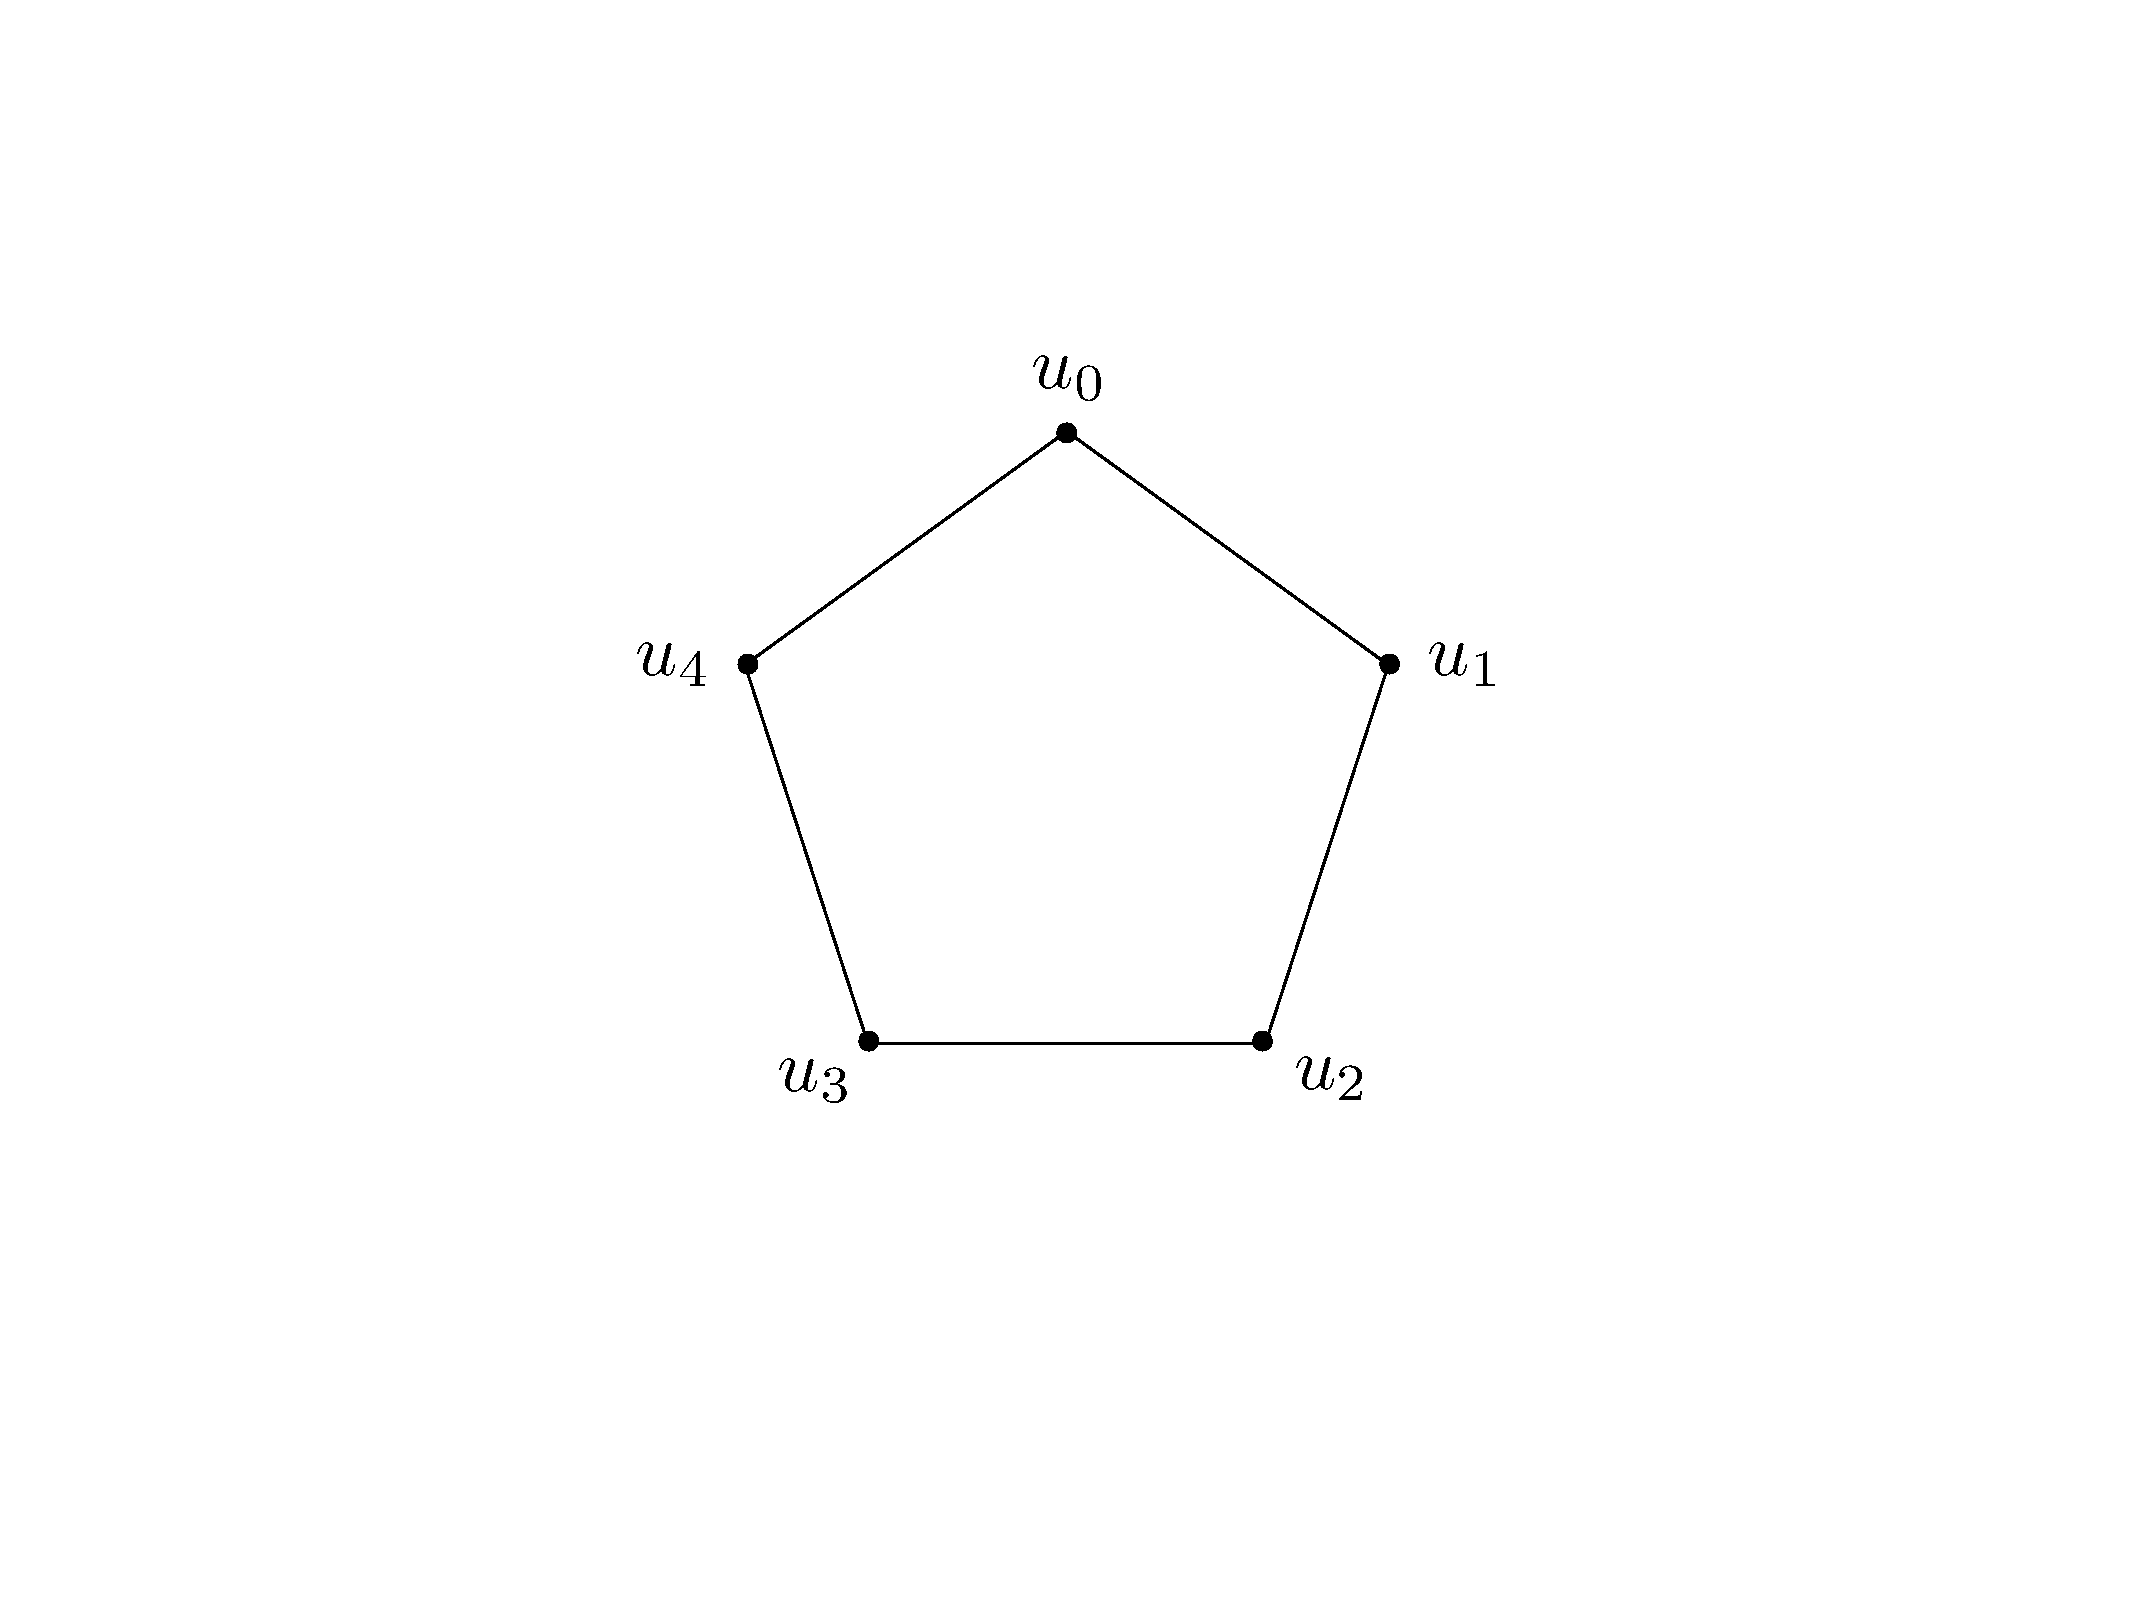
\includegraphics[scale=0.3]{dia1}
\end{center}
Sometimes we refer to this structure as a \emph{memory ring}.

Finally we take some commutative algebra structure on $\mathscr{V}$. The use of an algebra structure is implicit in \cite{ntm} and the deep learning literature in general, and enters  via the so-called \emph{Hadamard product} $\odot$ which makes $\mathbb{R}^n$ into an algebra via the rule
\begin{gather*}
\odot: \mathbb{R}^n \otimes \mathbb{R}^n \lto \mathbb{R}^n\,,\\
\bold{x} \odot \bold{y} = ( x_i y_i )_{i=1}^n\,.
\end{gather*}
We take $\mathscr{V} = \mathbb{R}^M$ with the Hadamard product in what follows. This involves choosing a basis, of course, but we will only refer to the product (a tensor $\odot \in \mathscr{V}^* \otimes \mathscr{V}^* \otimes \mathscr{V}$) and not the basis in what follows.

\begin{definition}[(Erase step)] Given a vector $e \in \mathscr{V}$ and a write address $w \in \mathscr{W}^*$ we define an action on the space of memory states $\mathscr{S}$ which we think of as ``erasing by $e$ at the address $w$'' as follows. Using
\[
\Psi( w \otimes e ) \in \Hom_{\mathbb{R}}(\mathscr{W}, \mathscr{V})
\]
we may form the composite
\[
\xymatrix@C+3pc{
\mathscr{W} \ar[r]^-{\Delta} & \mathscr{W} \otimes \mathscr{W} \ar[r]^-{M \otimes \Psi( w \otimes e )} & \mathscr{V} \otimes \mathscr{V} \ar[r]^-{m} & \mathscr{V}\,.
}
\]
\end{definition}

This is actually the multiplication in a canonical algebra structure on the space $\Hom_{\mathbb{R}}(\mathscr{W}, \mathscr{V})$ which arises from the fact that $\mathscr{W}$ is a coalgebra and $\mathscr{V}$ is an algebra. It is the \emph{convolution product} on the space of memory states. If we write
\[
M' = m \circ (M \otimes \Psi( w \otimes e )) \circ \Delta
\]
then 
\[
M'(e_i) = m \left( M(e_i) \otimes \Psi( w \otimes e )(e_i) \right) = M(e_i) \odot w(e_i) e\,.
\]
The space of memory states has a natural action of the cyclic group of order $N$, which acts by rotation on $\mathscr{W}$ and therefore on $\mathscr{S}$. The rotated state assigns the vector $u_{j+1}$ to the position $j$ (we index the positions in the clockwise order) with $j + 1$ computed modulo $N$. Said differently, let $R: \mathscr{W} \lto \mathscr{W}$ be the linear map defined by
\[
R( \overline{a} ) = \overline{a+1}\,,
\]
with dual map $R^*: \mathscr{W}^* \lto \mathscr{W}^*$. The rotation of the memory state $M$ is the composition $M \circ R$, or what is the same thing, $R^*( M )$. Thus, applying the $j$-th power of $R^*$ to a memory state has the effect of rotating the state $j$ times around the regular polygon.

The internal state space of the RNN underlying the NTM is decomposed as
\be\label{eq:decomp}
\mathscr{H} = \mathscr{H}_0 \oplus \mathscr{W} \oplus \mathscr{W}^* \oplus \mathscr{S}
\ee
and the state at time $t$ is written
\[
h^{(t)} = (h_0^{(t)}, r^{(t)}, w^{(t)}, M^{(t)}) \in \mathscr{H}\,.
\]
The components of this vector are interpreted as the \emph{controller internal state} $h_0^{(t)}$, \emph{read address weights} $r^{(t)}$, \emph{write address weights} $w^{(t)}$ and \emph{memory contents} $M^{(t)}$. For convenience we will refer to the read address weight as the \emph{read address}, even though the vector represents a distribution over the available addresses rather than a specific address. At each time step the RNN generates from its hidden state a distribution $s$ over rotations of the write address, a distribution $q$ over rotations of the read address, an operator $e$ to be applied to each coefficient vector in the memory state (this encodes ``forgetting'') and a vector $a$ to be written to memory, via the formulas
\begin{gather*}
s^{(t+1)} = \zeta( W_s h^{(t)} + B_s ) \in \mathscr{W}^*\,,\\
q^{(t+1)} = \zeta( W_q h^{(t)} + B_q ) \in \mathscr{W}^*\,,\\
e^{(t+1)} = \sigma( W_e h^{(t)} + B_e ) \in \mathscr{V}\,,\\
a^{(t+1)} = \sigma( W_u h^{(t)} + B_u ) \in \mathscr{V}\,.
\end{gather*}
The update equation for the addresses \cite[Eq. (8)]{ntm} and memory \cite[Eq. (3),(4)]{ntm} are
\begin{align}
w^{(t+1)} &= \sum_{i=0}^{N-1} s^{(t+1)}(\bar{i}) \cdot (R^*)^i( w^{(t)} )\,,\label{eq:ntm_update1}
\\
r^{(t+1)} &= \sum_{i=0}^{N-1} q^{(t+1)}(\bar{i}) \cdot R^i( r^{(t)} )\,,\label{eq:ntm_update2}\\
M^{(t+1)} &= (1_{\mathscr{V}} - e^{(t+1)} ) \circ M^{(t)} + w^{(t)} \otimes a^{(t+1)}\,.\label{eq:ntm_update3}
\end{align}
Finally, the evolution equation is
\be\label{eq:NTMequation}
h_0^{(t+1)} = \sigma\Big( M^{(t)}(r^{(t)}) + H_0 h_0^{(t)} + U_0 x^{(t+1)} + B_0 \Big)\,.
\ee 
where
\begin{gather*}
H_0: \mathscr{H}_0 \lto \mathscr{H}_0\,,\\
U_0: \mathscr{I} \lto \mathscr{H}_0\,,
\end{gather*}
and $B_0 \in \mathscr{H}_0$ are weight matrices. We assume for simplicity that the memory coefficient space is the same as the hidden state space, that is, $\mathscr{V} = \mathscr{H}$. Following \cite[\S 3.2]{ntm} we write $e$ for the \emph{erase vector} and $a$ for the \emph{add vector}. These equations define the NTM with location-based addressing, with an RNN controller and memory of size $N$ with a single read and write head.\footnote{We omit the sharpening step \cite[Eq. (9)]{ntm} for simplicity. The original NTM paper \cite{ntm} is not specific about how the output $M^{(t)}(r^{(t)})$ of the read heads enters the RNN evolution equation; the form we have given above follows the construction of the differentiable neural computer \cite[p. 7]{dnc}. Note that the term appearing in the equation for $h^{(t+1)}$ is the memory state at time $t$ applied to the output of the read heads at time $t$. That is, the output of the read heads is incorporated into the hidden state of the RNN at the \emph{next} time step; again, in this architectural choice we are following \cite{dnc}. Similarly, the write address used to define $M^{(t+1)}$ is $w^{(t)}$ rather than $w^{(t+1)}$. In this it seems we actually \emph{disagree} with \cite{ntm,dnc}. It makes the formulas cleaner, but maybe it is wrong (TODO). }

\begin{remark} To connect the above more explicitly to the notation of \cite[Eq. (8)]{ntm} observe that \eqref{eq:ntm_update2} can be rewritten, writing $r[j]$ for the component of $r \in \mathscr{W}$ for $\bar{j}$, as
\be\label{eq:moreexplicah}
r^{(t+1)}[i] = \sum_j q^{(t+1)}(\bar{j}) r^{(t)}[i-j]\,.
\ee
\end{remark}

\subsection{Linear Logic}

Linear logic is the universal way of describing algorithms which manipulate tensors and linear maps using the basic constructions of linear algebra (such as composition and tensor contraction) and iterations of such constructions. At the level of \emph{syntax} these algorithms may be thought of as programs written in a functional programming language much like the simply-typed lambda calculus. This programming language has a functorial \emph{semantics} denoted here by $\den{-}$ which realises the abstract algorithms as concrete functions.

In this section we give a very brief introduction to linear logic; for a longer survey see \cite{murfet_ll,murfetclift}. We divide the introduction into three parts, covering the \emph{types}, \emph{terms} (meaning programs) and \emph{semantics} of intuitionistic linear logic.

\subsubsection{Types}

The \emph{types} of intuitionistic linear logic are built from atomic types $\phi_1,\phi_2,\ldots$ via binary connectives $\otimes, \multimap$ (tensor, Hom) and a unary connective ${!}$ (called bang). Thus a type may be represented as a syntax tree, where the leaves are labelled by atomic types $\phi_i$ and the other vertices are labelled by $\otimes, \multimap, {!}$. For example the type
\[
{!}(\phi_1 \multimap \phi_1) \multimap (\phi_1 \multimap \phi_1)
\]
corresponds to the tree
\[
\xymatrix{
& & \multimap\\
& {!}\ar@{-}[ur] & & \multimap\ar@{-}[ul]\\
& \multimap\ar@{-}[u] & \phi_1\ar@{-}[ur] & & \phi_1\ar@{-}[ul]\\
\phi_1 \ar@{-}[ur] & & \phi_1 \ar@{-}[ul]
}
\]
Given a type $A$ we can construct two new types
\begin{align*}
\textbf{int}_A &= {!}(A \multimap A) \multimap (A \multimap A)\\
\textbf{bint}_A &= {!}(A \multimap A) \multimap \big({!}(A \multimap A) \multimap (A \multimap A)\big)
\end{align*}
called respectively the types of \emph{integers} on $A$ and \emph{binary integers} on $A$, which will play an important role in what follows.

\subsubsection{Terms}

There is a countable collection of variables $x_1^A,x_2^A,\ldots$ of each type $A$. Variables are \emph{terms} and a general term is built up from variables by a set \emph{deduction rules} which we will not review here, but which we will try to illuminate with examples. As usual we write $\pi: A$ to indicate that $\pi$ is a term of type $A$ and present terms as linear lambda terms, following \cite{benton_etal}. Some examples of linear lambda terms are, for variables $x:A,y:B$ and $z:{!} A$,
\begin{align}
(\lambda x \,.\, x) &: A \multimap A\,, \label{eq:example_lambda_1}\\
(\lambda x \,.\, (\lambda y \,.\, (y \; x))) &: A \multimap ((A \multimap A) \multimap A)\,,\label{eq:example_lambda_2}\\
(\lambda z \,.\, \operatorname{derelict}(z)) &: {!} A \multimap A\,. \label{eq:example_lambda_3}
\end{align} 

\begin{remark}\label{remark:atu} A term of type $A \multimap B$ should be thought of as a program which takes inputs of type $A$ and returns outputs of type $B$, under the constraint that the input is used \emph{linearly} (that is, precisely once). For example, the term \eqref{eq:example_lambda_1} just returns its input, while \eqref{eq:example_lambda_2} takes two inputs $x:A, y:A \multimap A$ and returns the result $(y \; x)$ of applying the second program to the first. In both cases the inputs are used linearly.

On the other hand a term of type ${!} A \multimap B$ is a program which takes inputs of type $A$ and returns outputs of type $B$, with no linearity constraint (so it is like a normal program in the lambda calculus). Usually such programs are constructed by first making copies of the input and then feeding those copies into a program, like those in \eqref{eq:example_lambda_1},\eqref{eq:example_lambda_2}, which is linear with respect to its inputs. To give such an example we need the \emph{dereliction} operator $\operatorname{derelict}(-)$ appearing in \eqref{eq:example_lambda_3} which takes an input which may be used arbitrarily ($z$ in our example) and returns a restricted form of the input which may only be used linearly.
\end{remark}

The simplest nontrivial example is the term (with $q:{!}(A \multimap A), z: A$)
\be\label{eq:church_2_linearlambda}
\underline{2} = (\lambda q.(\textrm{copy $q$ as $q',q''$ in } (\lambda z. (\derelict(q'') \; (\derelict(q')\; z)))))
\ee
which is of type 
\[
\underline{2}: \inta_A = {!}(A \multimap A) \multimap (A \multimap A)\,.
\]
Intuitively, this program takes an input $q: {!}(A \multimap A)$, copies it to form $q',q''$, and returns
\[
(\lambda z. (\derelict(q'') \; (\derelict(q')\; z)))
\]
which is itself a program, sending $z:A$ to what is intuitively the result of evaluating $q$ twice on $z$. The corrrect way to make this precise is as shown above, using the dereliction operator. In more informal language, the overall program $\underline{2}$ has the meaning $q \longmapsto q^2$.

Every term in intuitionistic logic can be interpreted as a linear map between (usually infinite-dimensional) vector spaces, and it is these interpretations (or \emph{denotations}, in the logic terminology) which will be used in the recurrent neural networks.

\subsubsection{Semantics}

The semantics $\den{-}$ of linear logic in the category $\cat{V}$ of vector spaces \cite[\S 5.1, \S 5.3]{murfet_ll} assigns to each type $A$ a vector space $\den{A}$ and to each term $\pi: A$ a vector $\den{\pi} \in \den{A}$ in a way which is compositional with respect to the structure of types and terms. We refer to the objects $\den{A}, \den{\pi}$ as the \emph{denotations} of $A,\pi$ respectively. 

The semantics depends on a choice, for each atomic type $\phi_i$, of a vector space $\den{\phi_i}$. This choice is made freely and once made, determines all denotations, according to the following inductive definitions:
\begin{align*}
\den{A \multimap B} &= \Hom_k(\den{A},\den{B})\,,\\
\den{A \otimes B} &= \den{A} \otimes \den{B}\,,\\
\den{{!}A} &= {!} \den{A}\,,
\end{align*}
where $\Hom_{\mathbb{R}}(W,V)$ is the space of linear maps from $W$ to $V$ (we will also use the notation $\End_{\mathbb{R}}(V) = \Hom_{\mathbb{R}}(V,V)$). Here ${!} V$ denotes the universal cocommutative counital coalgebra mapping to $V$, or what is the same, the space of distributions with finite support on (a finite-dimensional subspace of) $V$ viewed as a smooth manifold. This is a bit complicated to describe, but it suffices here to know that there is a canonical (non-linear!) function
\be\label{eq:vtobangv}
V \lto {!} V\,, \qquad u \longmapsto \ket{\emptyset}_u
\ee
sending a vector $u \in V$ to the Dirac distribution concentrated at $u$.

\begin{example}\label{example:denotation_intaphi} The vector space
\begin{align*}
\den{{!}( \phi_1 \multimap \phi_1 ) \multimap (\phi_1 \multimap \phi_1) } &= \Hom_{\mathbb{R}}( \den{{!}(\phi_1 \multimap \phi_1)}, \den{\phi_1 \multimap \phi_1})\\
&= \Hom_{\mathbb{R}}( {!} \End_{\mathbb{R}}(\den{\phi_1}), \End_{\mathbb{R}}(\den{\phi_1}))
\end{align*}
is determined once $\den{\phi_1}$ is. The construction can be understood in terms of the tree \eqref{??} by starting with the vector space $\den{\phi_1}$ at the leaves and combining these vector spaces according to the operations at the vertices.
\end{example}

Having explained how the denotations of types are defined, we now turn to denotations of terms. For any term $\pi$ of type $A$ the denotation is a vector $\den{\pi} \in \den{A}$. In particular, if $\rho$ is of type $A \multimap B$ then its denotation is a vector
\[
\den{\rho} \in \den{A \multimap B} = \Hom_{\mathbb{R}}(\den{A}, \den{B})
\]
that is, the denotation is a linear map $\den{A} \lto \den{B}$. Similarly, if $\gamma$ is of type ${!}A \multimap B$ then its denotation is a linear map
\[
\den{\gamma}: {!} \den{A} \lto \den{B}\,.
\]
In Remark \ref{remark:atu} we explained how to think of both $\rho, \gamma$ as programs taking inputs of type $A$, but where $\rho$ is restricted to use this input linearly. In the semantics this resolves to the distinction between $\den{A}$ and ${!} \den{A}$. We can still think of $\den{\gamma}$ as taking inputs of type $A$ (i.e. vectors in $\den{A}$) using \eqref{eq:vtobangv} to define the (non-linear) composite
\be\label{eq:defnnl}
\xymatrix@C+2pc{
\den{A} \ar[r] & {!} \den{A} \ar[r]^-{\den{\gamma}} & \den{B}
}
\ee
which feeds $u \in \den{A}$ to $\den{\gamma}$. This composite is denoted $\den{\gamma}_{nl}$, see \cite[Definition 5.10]{murfet_ll}.

We will not describe here the precise rules which construct the denotations of terms, but illustrate the idea with examples from \cite[\S 3]{murfetclift}. We fix a type $A$ and set $V = \den{A}$.

%The most elementary form of iteration is repetition. The simplest example of this form of iteration in the current context is raising a linear operator to an integer power. This non-linear transformation of an input operator $\alpha \in \End_{\mathbb{R}}(\mathscr{H})$ to the output operator $\alpha^n$ is encoded by a proof $\underline{n}$ in linear logic of the type
% where $\den{A} = \mathscr{H}$. A more interesting kind of iteration takes a pair of linear operators $\alpha, \beta$ and intertwines them according to a sequence of binary numbers $S \in \{0,1\}^*$. This transformation is encoded by a proof $\underline{S}$ in linear logic of type
% We begin this section with a brief exposition on the iterators $\underline{n}$ and $\underline{S}$ before going on to explain how they appear in various special cases of the LLRNN. The iterator $\underline{n}$ is the basic tool in the linear logic implementation of the NTM (Section \ref{example:ntm}) and its generalisations in Section \ref{example:ntm_extended} and Section \ref{example:ntm_super} while the iterator $\underline{S}$ is used in Example \ref{example:dihedral}. 

\begin{example}\label{example_1} The denotation of a term $\pi$ of type $\textbf{int}_A$ is by Example \ref{example:denotation_intaphi} a vector
\[
\den{\pi} \in \den{\inta_A} = \Hom_{\mathbb{R}}( {!} \End_{\mathbb{R}}(V), \End_{\mathbb{R}}(V))\,.
\]
Thus $\den{\pi}$ is a linear map ${!} \End_{\mathbb{R}}(V) \lto \End_{\mathbb{R}}(V)$. For each integer $n \ge 0$ there is a term $\underline{n}$ of type $\inta_A$, with $\underline{2}$ being given already in \eqref{??}. One calculates that for $\alpha \in \End_{\mathbb{R}}(V)$,
\[
\den{\underline{n}} \ket{\emptyset}_\alpha = \alpha^n.
\]
Another way to express this is to say that the non-linear function
\[
\den{\pi}_{nl}: \End_{\mathbb{R}}(V) \lto \End_{\mathbb{R}}(V)
\]
satisfies $\den{\underline{n}}_{nl}(\alpha) = \alpha^n$. %To be clear, writing $\mathscr{K} = \mathbb{R}^{n_H}$ and identifying $\End_{\mathbb{R}}(\mathscr{K})$ with the space of matrices $M_{n_H}(\mathbb{R})$, the denotation of any proof of $\textbf{int}_\alpha$ will be a function $\den{\pi}(X)_{ij}: M_{n_H}(\mathbb{R}) \lto \mathbb{R}$ which is a polynomial in the entries $X_{kl}$ for $1 \le i, j \le n_H$.
\end{example}

\begin{example}\label{example_2} The denotation of a proof $\pi$ of type $\textbf{bint}_A$ gives a function
\[
\den{\pi}_{nl}: \End_{\mathbb{R}}(V) \times \End_{\mathbb{R}}(V) \lto \End_{\mathbb{R}}(V)\,.
\]
For every binary sequence $S \in \{0,1\}^*$ there is a corresponding term $\underline{S}$ of type $\binta_A$ \cite[\S 3.2]{murfetclift}. For example
\[
\underline{001} = (\lambda q.(\lambda p.(\textrm{copy $q$ as $r,s$ in } (\lambda z.(\derelict(p)\;(\derelict(s)\;(\derelict(r)\;z)))))))\,.
\]
The denotation $\den{\underline{S}}_{nl}$ sends a pair of linear operators $\alpha,\beta$ to the product described by $S$, reading $\alpha$ for $0$ and $\beta$ for $1$, and reading in reverse order. For example,
\[
\den{\underline{001}}_{nl}(\alpha,\beta) = \beta \alpha \alpha\,.
\]
\end{example}

\section{The Linear Logic Recurrent Neural Network}

There is a class of augmented RNNs with the following general form: at each time step a linear operator on the hidden state space
\[
Z = Z(h^{(t)}, x^{(t+1)}) \in \End_{\mathbb{R}}(\mathscr{H})
\]
is generated from the previous hidden state and current input, and then this linear operator $Z$ is applied to the hidden state to generate a vector $Z(h^{(t)})$ which is inserted into the RNN evolution equation for $h^{(t+1)}$. Both the second-order RNN \eqref{??} and NTM \eqref{??} have this general form. What is the \emph{generic} augmented RNN of this kind? 

Obviously $Z$ should be a (piece-wise) differentiable function of the hidden state and current input, but we consider a more restricted class of functions constructed as follows: in the first step, using feed-forward neural networks, we generate from $h^{(t)}, x^{(t+1)}$ a family of vectors (keeping in mind that tensors and linear operators are also vectors). In the second step, these vectors are combined algorithmically using iteration and the basic operations of linear algebra to produce the linear operator $Z$. The vectors generated in the first step are called \emph{command vectors}, \emph{data vectors} or \emph{input vectors}, depending on how they are constructed (see below for details). The algorithmic construction in the second step is a fixed linear logic program which we refer to as the \emph{master algorithm}. The generic augmented RNN defined in this way is called the Linear Logic RNN (LLRNN).

In fact it is natural to consider two linear operators $Z_{\operatorname{in}}, Z_{\operatorname{out}}$, with the former appearing within the evolution equation \emph{inside} the nonlinearity and the latter appearing \emph{outside} the nonlinearity. Thus the evolution equation of the LLRNN model is
\be\label{eq:masterh}
h^{(t+1)} = \sigma\Big( Z_{\mathrm{in}}(h^{(t)}) + H h^{(t)} + U x^{(t+1)} + B\Big) + Z_{\mathrm{out}}(h^{(t)})
\ee
where the linear operators $Z_z \in \End_{\mathbb{R}}(\mathscr{H})$ for $z \in \{\mathrm{in},\mathrm{out}\}$ depend on $h^{(t)}, x^{(t+1)}$ via the aforementioned feed-forward networks
\begin{align*}
p_i^{(t+1)} &= \zeta( W^p_i h^{(t)} + B^p_i ) \in \mathscr{P}_i\,, \qquad 1 \le i \le r\,,\\
b_j^{(t+1)} &= \sigma( W^b_j h^{(t)} + B^b_j ) \in \mathscr{B}_j\,, \qquad 1 \le j \le s\,,\\
c^{(t+1)} &=  W^c x^{(t+1)} \in \mathscr{C}\,.
\end{align*}
and the denotation of a term $\master^z$ in linear logic, via the formula
\be\label{eq:masterz}
Z_z = \den{\underline{\mathrm{master}}^z}_{nl}\Big( p_1^{(t+1)}, \ldots, p_r^{(t+1)}, b_1^{(t+1)}, \ldots, b_s^{(t+1)}, c^{(t+1)}\Big)\,.
\ee
Here we use that the denotation $\den{\master^z}$ defines a differentiable function
\be
\mathscr{P}_1 \times \cdots \times \mathscr{P}_r \times \mathscr{B}_1 \times \cdots \times \mathscr{B}_s \times \mathscr{C} \lto \End_{\mathbb{R}}(\mathscr{H})\,.
\ee
We give the vectors generated in the first step names; we have

% At each time step the second-order RNN generates from its input a linear operator which is applied to to the hidden state; this operator moreover depends \emph{linearly} on the input. The LLRNN model is similar in that it generates at each time step a linear operator which is applied to the hidden state, but dissimilar in that this operator depends \emph{non-linearly} on the input as well as a sequence of other vectors generated from the hidden state.

% The non-linear function which computes the operator to be applied to the hidden state at each time step is called the \emph{master algorithm}. It is itself the denotation of a proof in linear logic. The arguments to the master algorithm are:
\begin{itemize}
\item A sequence of \emph{command vectors} $p_i^{(t+1)}$ generated via softmax $\zeta$ from $h^{(t)}$,
\item a sequence of \emph{data vectors} $b_i^{(t+1)}$ generated via $\sigma$ from $h^{(t)}$,
\item an \emph{input vector} $c^{(t+1)}$ generated via $\sigma$ from $x^{(t+1)}$.
\end{itemize}
The idea is that the command vectors give distributions over finite-dimensional spaces of linear logic programs, while the data vectors and input vector give the inputs to be fed in some way into the selected programs; the exact details of this ``feeding'' are specified by the master algorithm. 

\begin{definition} The Linear Logic Recurrent Neural Network (LLRNN) is determined by the following data:
\begin{itemize}
\item types $P_1,\ldots,P_r$ called the \emph{command types};
\item types $B_1,\ldots,B_s$, called the \emph{data types};
\item a type $C$, called the \emph{input type};
\item a type $A$ with $\den{A} = \mathscr{H}$, the hidden state space;
\item two proofs $\underline{\mathrm{master}}^z$ for $z \in \{\mathrm{in},\mathrm{out}\}$ of the sequent
\be
{!} P_1, \ldots, \, {!}P_r,\, {!} B_1, \ldots,\, {!} B_s,\, {!} C \vdash A \multimap A\,.
\ee
\item Finite-dimensional subspaces for $1 \le i \le r$ and $1 \le j \le s$
\be
\mathscr{P}_i \subseteq \den{P_i}\,, \quad \mathscr{B}_j \subseteq \den{B_j}\,, \quad \mathscr{C} \subseteq \den{C}
\ee
which are spanned by the denotations of linear logic proofs. We refer to the elements of $\mathscr{P}_i$ as \emph{command vectors}, elements of $\mathscr{B}_j$ as \emph{data vectors} and elements of $\mathscr{C}$ as \emph{input vectors}.
\end{itemize}
\end{definition}

The fundamental fact which makes this model reasonable is the following:

\begin{proposition} The functions $\den{\master^z}_{nl}$ are smooth.
\end{proposition}
\begin{proof}
This follows from the hypothesis that $\mathscr{P}_i, \mathscr{B}_j$ are generated by denotations of linear logic proofs, and the smoothness of these denotations \cite{murfetclift}.
\end{proof}

Moreover, the derivatives of $\den{\master^z}_{nl}$ can be computed symbolically using the cut-elimination algorithm of differential linear logic, and it is therefore feasible to implement a general LLRNN in a software package like TensorFlow. 

\begin{remark}\label{remark:sequentbang} It will often be convenient to write $\Gamma = P_1, \ldots, P_r$ for the command types and $\Delta = B_1, \ldots, B_s$ for the data types. A standard notational device in the linear logic literature is to then write ${!} \Gamma$ for the list preprending ${!}$ to all the types in the list $\Gamma$, that is, ${!} \Gamma = {!} P_1, \ldots, {!} P_r$. With this notation, $\master$ is a proof of ${!} \Gamma, {!} \Delta, {!} V \vdash A \multimap A$.
\end{remark}

\subsection{Examples}

As defined the LLRNN is a class of models. In this section we explain how to implement various existing augmentations of RNNs, including a subset of the Neural Turing Machine, in the framework of the LLRNN. The guiding intuition from logic is that the complexity of an algorithm is rooted in the kind of \emph{iteration} that it employs; for an exposition in the context of linear logic see \cite[\S 7]{murfet_ll}. From this point of view, the purpose of augmenting an RNN with linear logic is to provide access to iterators of a complexity ``similar'' to the function that the neural network is trying to approximate.

\begin{example}[(Second-order RNN)] With $r = s = 0$ there are no command or data vectors. Take for the input type $C = A \multimap A$ and
\[
\mathscr{C} = \End_{\mathbb{R}}(\mathscr{H}) = \den{A \multimap A}\,.
\]
so the master algorithm takes a single input, which is a linear operator on the hidden state, and returns such an operator. The only weight matrix involved in the LLRNN beyond the usual RNN is the matrix $W^c$ which maps inputs to linear operators on $\mathscr{H}$.

We choose $\master^{\mathrm{in}}$ to be the proof of ${!}(A \multimap A) \vdash A \multimap A$ which is given by dereliction, so that $\den{\master^{\mathrm{in}}}_{nl}(\alpha) = \alpha$ and hence
\be\label{eq:secondorderRNNinLLRNN}
Z_{\mathrm{in}} = W^c(x^{(t+1)})\,.
\ee
Thus the LLRNN with these settings is just the second-order RNN.
\end{example}

The most elementary coupling of an RNN to linear logic adds the ability to raise linear operators (generated say from an input symbol, in the manner of the second-order RNN) to a power generated from the hidden state of the RNN. 

\begin{example}[(Higher-order RNN)] Consider the generalisation of the second-order RNN where the controller predicts at each time step an integer power of the linear operator $W^c(x^{(t+1)})$ to apply to the hidden state. Suppose we allow powers in the range $\{0,\ldots,L\}$. Then at each time step the RNN will generate a distribution $p^{(t+1)}$ over $\{0,\ldots,L\}$ from the current hidden state $h^{(t)}$ by the formula
\[
p^{(t+1)} = \zeta( W_p h^{(t)} + B_p )
\]
and therefore
\be\label{eq:higherorderRNN}
Z_{\operatorname{in}} = \sum_{i=0}^L p_i^{(t+1)} \big( W^c(x^{(t+1)}) \big)^i\,.
\ee
The operation of taking a linear operator and raising it to the $n$th power is encoded by the proof $\underline{n}$ of type $\inta_A$. We can therefore represent the higher-order RNN as a LLRNN, as follows. There is one command type $\inta_A$, no data types, and input type $A \multimap A$. The spaces of command and input vectors are respectively
\begin{align*}
\mathscr{P}_1 &= \operatorname{span}(\den{\underline{0}}, \ldots, \den{\underline{L}}) \subseteq \den{\inta_A}\,,\\
\mathscr{C} &= \End_{\mathbb{R}}(\mathscr{H}) = \den{A \multimap A}\,.
\end{align*}
We omit $\master^{\mathrm{out}}$ and take $\master^{\mathrm{in}}$ to be the proof of
\[
{!}\inta_A, \, {!}(A \multimap A) \vdash A \multimap A
\]
given in the term calculus of \cite{benton_etal} by
\[
\master^{\mathrm{in}} = (\lambda n. (\lambda a. (\derelict(n) \; a)))\,.
\]
This proof has the property that for $n_i \ge 0$ and $\alpha \in \End_{\mathbb{R}}(\mathscr{H})$ and $p_i \in \mathbb{R}$,
\be
\den{\master^{\mathrm{in}}}_{nl}\big( \sum_i \lambda_i \den{\underline{n}_i}, \alpha \big) = \sum_i \lambda_i \alpha^{n_i}\,.
\ee
The coupling of this function to the RNN is via $p_1^{(t+1)}$ which we identify with $p^{(t+1)}$ above, and $c^{(t+1)} = W^c(x^{(t+1)})$. By construction the LLRNN with this configuration reproduces the $Z$ of \eqref{eq:higherorderRNN} and thus the higher-order RNN.
\end{example}

Since one doesn't need to know linear logic to understand how to raise a linear operator to an integer power, it is natural to wonder to what degree linear logic is actually necessary here. All of our models can be formulated without any mention of linear logic, and indeed we will generally present the functions $\den{\master}_{nl}$ rather than the underlying proof. Nonetheless, the construction of $\master$ within linear logic constrains the model and makes conceptually clear the computational ideas involved; these ideas are not necessarily clear from the polynomial algebra that results from applying the denotation functor $\den{-}$. The strongest example of this point of view is the role of iteration in the LLRNN approach to the Neural Turing Machine and its generalisations.

\subsection{NTM as an LLRNN}\label{section:ntmasllrnn}

We now explain how to present the NTM of Section \ref{example:ntm} as an LLRNN. We first give the command, data and input types. Let $V,W$ be types of linear logic with $\den{V} = \mathscr{V}, \den{W} = \mathscr{W}$, and write $W^{\vee} = W \multimap 1$ so that $\den{W^{\vee}} = \mathscr{W}^*$. The command types $\Gamma$ and data types $\Delta$ are defined to be respectively
\[
\Gamma = \inta_W, \inta_{W^{\vee}}\,, \qquad \Delta = W \multimap W, W^{\vee} \multimap W^{\vee}, V \multimap V, V\,.
\]
The master algorithms are the proofs of ${!} \Gamma, {!} \Delta \vdash A \multimap A$ such that for inputs
\begin{gather*}
\den{\underline{m}} \in \den{\inta_W}\,,\quad \den{\underline{n}} \in \den{\inta_{W^{\vee}}}\,\\
\alpha \in \den{ W \multimap W} = \End_{\mathbb{R}}(\mathscr{W})\,\\
\beta \in \den{ W^{\vee} \multimap W^{\vee}} = \End_{\mathbb{R}}(\mathscr{W}^*)\,\\
e \in \den{V \multimap V} = \End_{\mathbb{R}}(\mathscr{V})\,\\
a \in \den{V} = \mathscr{V}
\end{gather*}
we have, for $h = (h_0,r,w,M) \in \mathscr{H}$ decomposed according to \eqref{eq:decomp},
\begin{align*}
\den{\master^{\mathrm{in}}}_{nl}\big( \den{\underline{m}}, \den{\underline{n}}, \alpha, \beta, e, a )(h) &= \big( M(r), 0, 0, 0 \big)\,,\\
\den{\master^{\mathrm{out}}}_{nl}\big( \den{\underline{m}}, \den{\underline{n}}, \alpha, \beta, e, a )(h) &= \big( 0, \alpha^m(r), \beta^n(w), (1_{\mathscr{V}} - e ) \circ M + w \otimes a\big)\,.
\end{align*}
As before we take $\mathscr{V} = \mathscr{H}$. We take
\begin{gather*}
\mathscr{P}_1 = \operatorname{span}(\den{\underline{0}}, \ldots, \den{\underline{N-1}}) \subseteq \den{\inta_W}\,,\\
\mathscr{P}_2 = \operatorname{span}(\den{\underline{0}}, \ldots, \den{\underline{N-1}}) \subseteq \den{\inta_{W^{\vee}}}\,,\\
\mathscr{B}_1 = \den{ W \multimap W} = \End_{\mathbb{R}}(\mathscr{W})\,,\\
\mathscr{B}_2 = \den{ W^{\vee} \multimap W^{\vee}} = \End_{\mathbb{R}}(\mathscr{W}^*)\,,\\
\mathscr{B}_3 = \den{ V \multimap V} = \End_{\mathbb{R}}(\mathscr{V})\,\\
\mathscr{B}_4 = \den{V} = \mathscr{V}\,.
\end{gather*}
We restrict the functions $\den{\master^z}_{nl}$ to the subset of inputs where $\alpha = R, \beta = R^*$. The coupling of this restricted function to the RNN is via command vectors $p_1^{(t+1)}, p_2^{(t+1)}$ giving distributions over the basis $\{ \den{\underline{i}} \}_{i=0}^{N-1}$ of $\mathscr{P}_1,\mathscr{P}_2$ which we identify respectively with $q^{(t+1)}$ (the distribution over powers of $R$ used to manipulate the read address) and $s^{(t+1)}$ (the distribution over powers of $R^*$ used to manipulate the write address).

We assume the weight matrix $H$ of \eqref{eq:masterh} is the projection from $\mathscr{H}$ to $\mathscr{H}_0$ followed by the weight $H_0$ above, and similarly for $U,B$. Then with the current notation the evolution equation \eqref{eq:masterh} of the LLRNN reads
\begin{align*}
(h_0^{(t+1)}, r^{(t+1)}, w^{(t+1)}, M^{(t+1)}) &= \Big( \sigma\big( M^{(t)}(r^{(t)}) + H_0 h_0^{(t)} + U_0 x^{(t+1)} + B_0 \big)\,,\\
&\qquad \sum_{i=0}^{N-1} (p_1^{(t+1)})_i R^i( r^{(t)} )\,, \sum_{i=0}^{N-1} (p_2^{(t+1)})_i (R^*)^i( w^{(t)} )\,,\\
&\qquad (1_{\mathscr{V}} - e^{(t+1)} ) \circ M^{(t)} + w^{(t)} \otimes a \Big)\,,
\end{align*}
which agrees with the equations \eqref{eq:ntm_update1} -- \eqref{eq:NTMequation}.

\begin{example}[(Dihedral NTM)]\label{example:dihedral} The NTM manipulates its memory state via rotations of the regular $N$-gon. In this example we study the natural extension which allows access the full symmetry group, the dihedral group, by adding the reflection
\begin{gather*}
R': \mathscr{W} \lto \mathscr{W}\,,\\
R'(\overline{a}) = \overline{-a}.
\end{gather*}
Note that $R'$ and $R$ do not commute. The command and data types are now
\begin{gather*}
\Gamma = \binta_W, \binta_{W^{\vee}}\,,\\
\Delta = W \multimap W, W \multimap W, W^{\vee} \multimap W^{\vee}, W^{\vee} \multimap W^{\vee}, V \multimap V, V
\end{gather*}
and $\master^{\mathrm{out}}$ is the proof such that for $h \in \mathscr{H}$ and $F,G \in \{0,1\}^*$
\begin{align*}
\den{\master^{\mathrm{out}}}_{nl}&\big( \den{\underline{F}}, \den{\underline{G}}, \alpha_1, \alpha_2, \beta_1, \beta_2, e, a )(h)\\
& = \Big(M(r), \den{F}_{nl}(\alpha_1,\alpha_2)(r),\den{G}_{nl}(\beta_1,\beta_2)(w), (1_{\mathscr{V}} - e) \circ M + w \otimes a\Big)\,.
\end{align*}
We then fix $\alpha_1 = R, \alpha_2 = R'$ and $\beta_1 = R^*, \beta_2 = (R')^*$.
\end{example}

\section{Generalisations of the NTM}

% The Differentiable Neural Computer (DNC) \cite{dnc} generalises the NTM by allowing for more complicated patterns of memory access based on a probabilistic incidence matrix $L[i,j]$ which records when positions in memory are written in successive time steps. An alternative approach to allowing more complicated memory access patterns is a more thoroughgoing use of iterators; this is more in keeping with the spirit of the LLRNN, and is the perspective we explore in the next section.

Taking the linear logic point of view on the NTM from Section \ref{section:ntmasllrnn} as a starting point, we develop several generalisations. The main purpose of these models is to demonstrate how a high-level idea for extending the basic NTM model can be realised by first translating the idea into linear logic, and then using the LLRNN form of the NTM.

\subsection{Pattern NTM}\label{example:ntm_extended}

At each time step the NTM predicts distributions $s^{(t)}, q^{(t)}$ over the possible rotations of the write and read addresses. A pattern of memory accesses is a \emph{sequence} of such rotations, and since the ``angle'' of rotation is represented in the LLRNN as the denotation of a linear logic proof (with $\den{\underline{n}}$ representing a clockwise angle of $\frac{2\pi n}{5}$) the pattern may be stored as a sequence of vectors in $\den{\inta_W}$. It is therefore natural to add a memory ring with coefficients in this vector space, which in principle should allow the NTM to learn more complex patterns of memory access. In this example we first present the construction using linear logic, and then afterward translate this into explicit equations involving matrices.

Let $\mathfrak{a} = \{a,b,\ldots,z\}$ and let $\mathscr{V}_1 = \oplus_{i \in \mathfrak{a}} \mathbb{R} i$ be the free vector space on $A$. We also take a finite-dimensional subspace $\mathscr{V}_2 \subseteq \den{\inta_W}$. For convenience we keep the same address space for both memory rings. So we have memory spaces for $i \in \{1,2\}$
\[
\mathscr{S}_i = \mathscr{W}^* \otimes \mathscr{V}_i \cong \Hom_{\mathbb{R}}(\mathscr{W}, \mathscr{V}_i)\,.
\]
An example of a combined state $\mathscr{S} = \mathscr{S}_1 \oplus \mathscr{S}_2$ of these two memory spaces is
\begin{center}
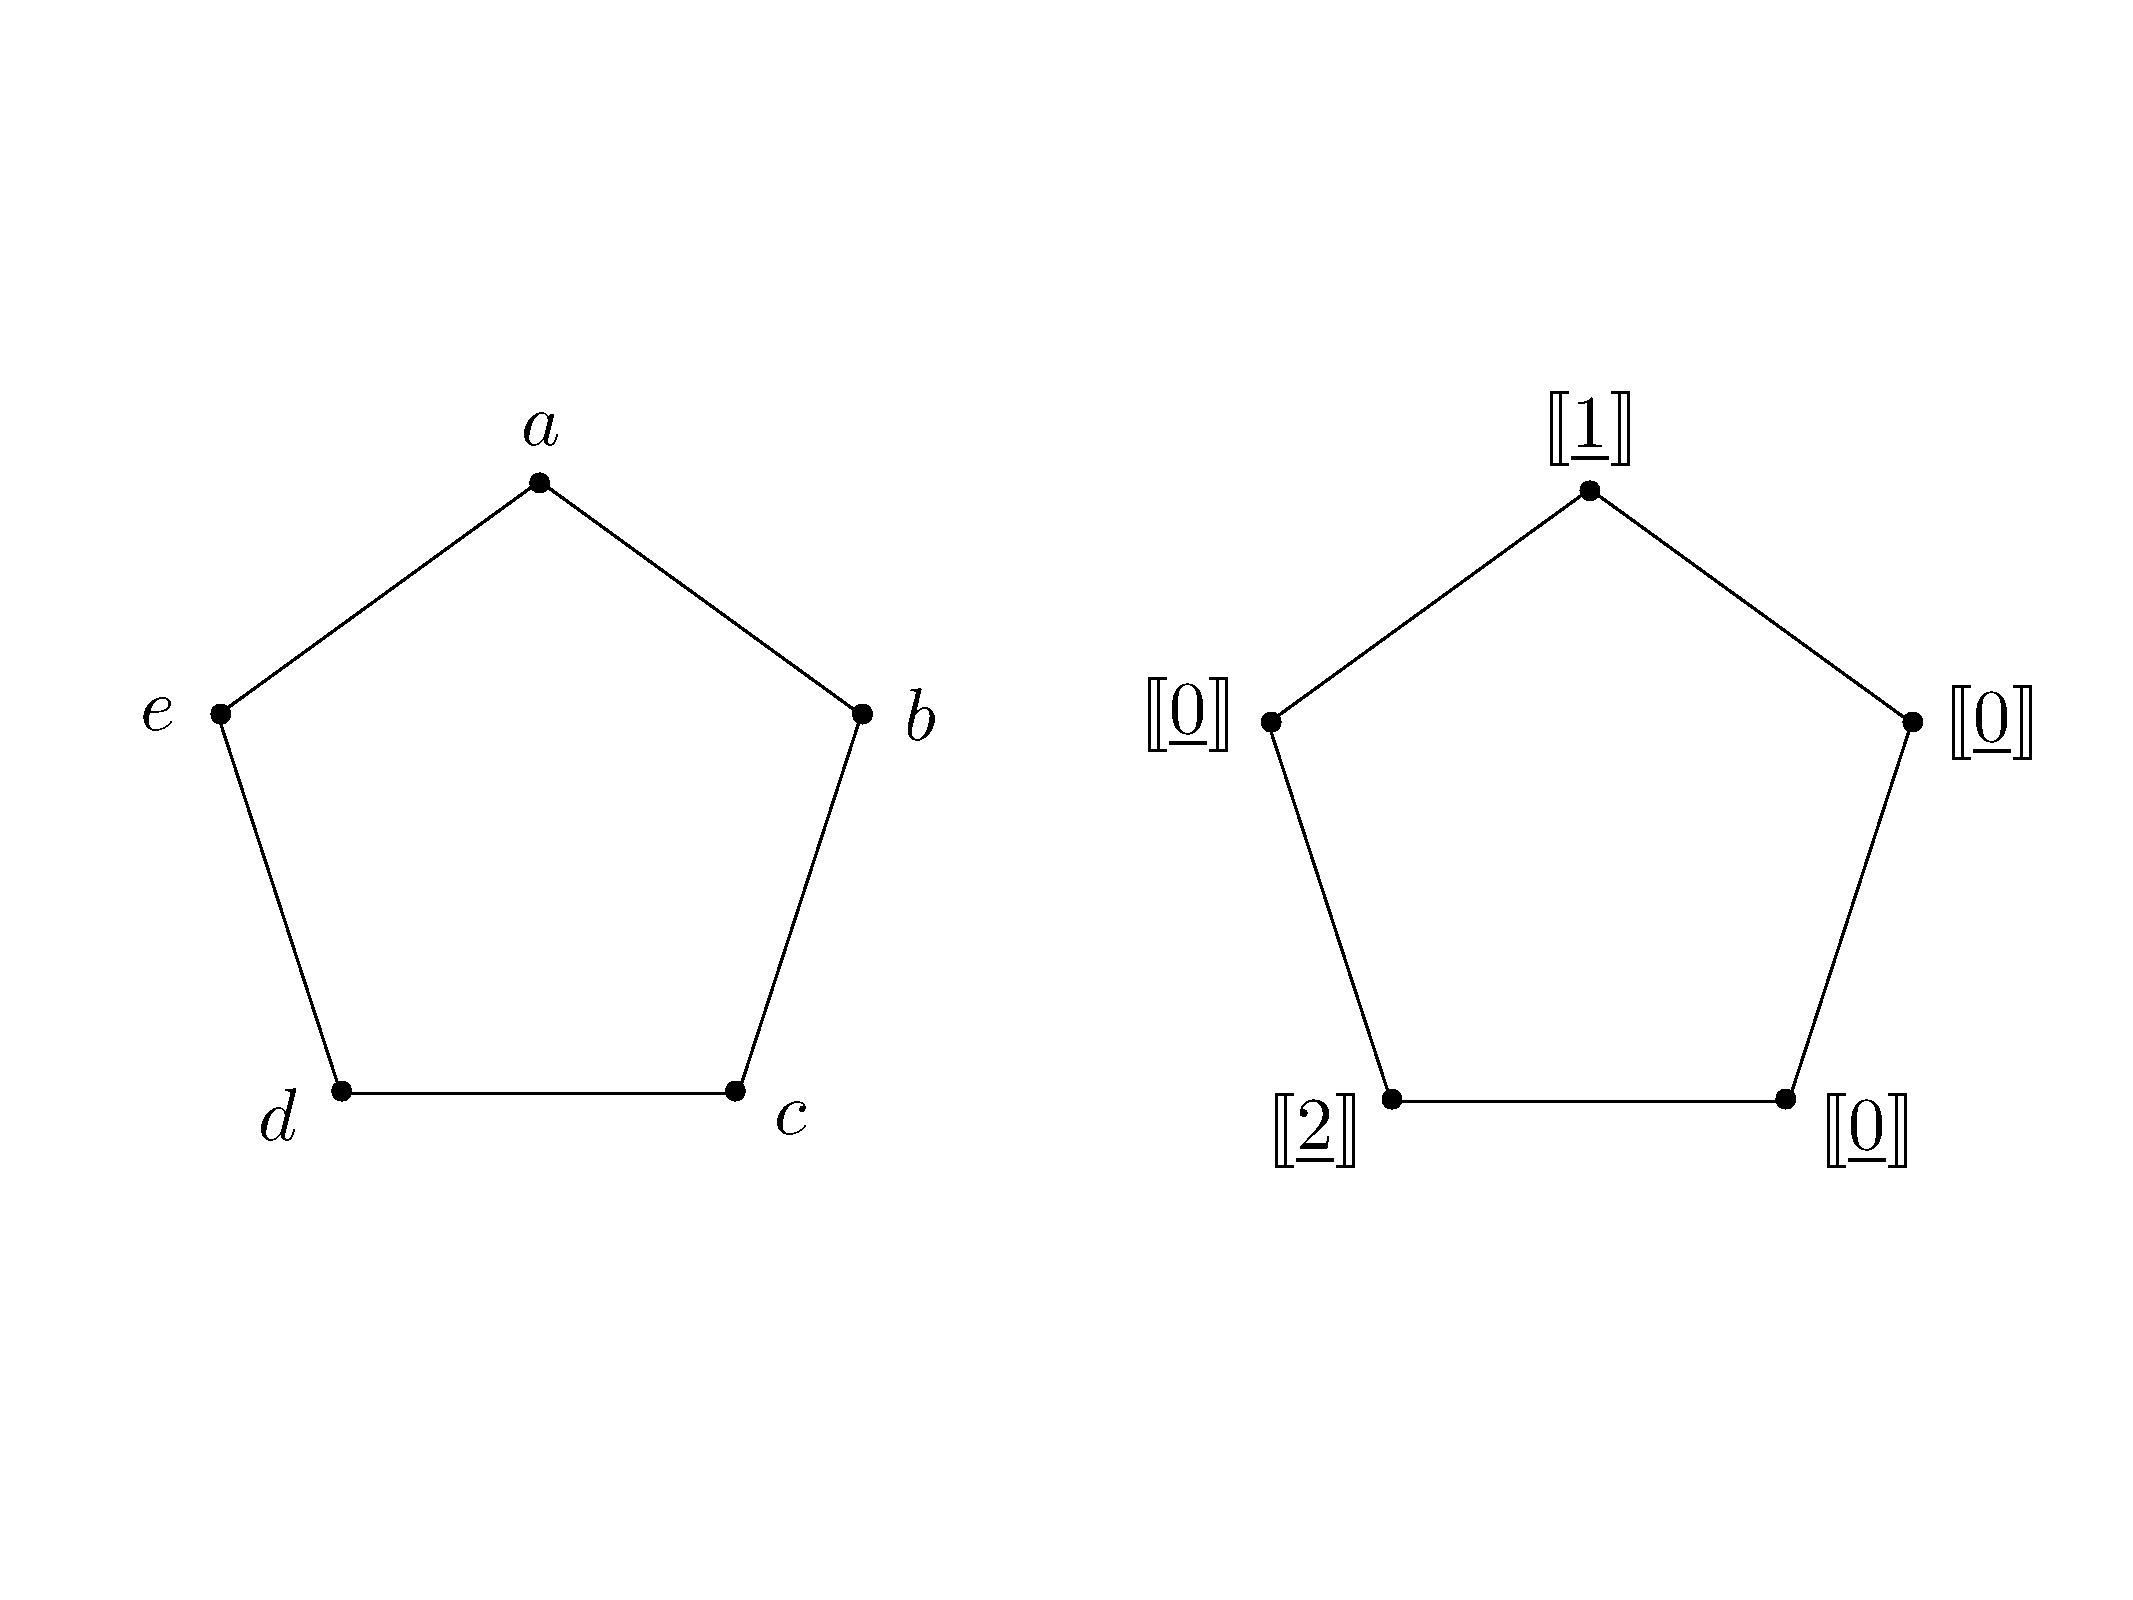
\includegraphics[scale=0.3]{dia2}
\end{center}
We consider a modification of the NTM in which the contents of the second ring control the motion of the read address of the first ring (rather than this being manipulated directly by the RNN controller). To demonstrate the dynamics in an example, suppose that the memory state is as shown at time $t = t_0$, that the read address for the first ring is focused at the zero position at time $t_0 - 1$, and that the read address for the second ring is focused at zero at time $t_0$ and increases its focus position by one step over each time interval. 

Then as time increases from $t_0$ the repeating sequence
\be\label{eq:deliver_iterators}
\den{\underline{1}}, \den{\underline{0}}, \den{\underline{0}}, \den{\underline{0}}, \den{\underline{2}}, \den{\underline{0}}, \ldots
\ee
will be used to control the read address of the first memory ring. More precisely, the operator applied to the read address $r_1 \in \mathscr{W}$ will be $R^n$ with $n$ varying over the repeating sequence $1,0,0,2,0$. Finally, the sequence of vectors delivered to the controller will be
\[
a, b, b, b, d, d, e, e, e, b, \ldots\,.
\]
In more detail, as part of $\master$ there will be an evaluation program
\[
\begin{mathprooftree}
\AxiomC{$\underline{\mathrm{eval}}$}
\noLine\UnaryInfC{$\vdots$}
\def\extraVskip{5pt}
\noLine\UnaryInfC{$\inta_W, {!}(W \multimap W) \vdash W \multimap W$}
\end{mathprooftree}
\]
which has the property that
\[
\den{\underline{\mathrm{eval}}}\big( \sum_i \lambda_i \den{\underline{n}_i}, \ket{\emptyset}_\alpha \big) = \sum_i \lambda_i \alpha^{n_i}\,.
\]
The first argument to this evaluation function will be the state $M_2(r_2) = \sum_i \lambda_i \den{\underline{n}_i}$ of the second memory ring. We apply the output to the read address $r_1$ of the first memory ring and specialise to $\alpha = R$ so that the relevant expression is
\[
\den{\underline{\mathrm{eval}}}( M_2(r_2), \ket{\emptyset}_R )(r_1) = \sum_i \lambda_i R^{n_i}(r_1)\,.
\]
The command and data types are
\begin{gather*}
\Gamma = \inta_{W^{\vee}}, \inta_W, \inta_{W^{\vee}}\,\\
\Delta = W \multimap W, W^{\vee} \multimap W^{\vee}, W \multimap W, W^{\vee} \multimap W^{\vee}, V \multimap V, V, \inta_W \multimap \inta_W, \inta_W\,.
\end{gather*}
The first type in $\Gamma$ is connected to the write address for the first memory ring, while the second and third types relate respectively to the read and write address of the second memory ring. We do not include an input to the master algorithm for manipulating the read address of the first memory ring since this is purely under the control of the second memory ring. The inputs of type $V \multimap V, V$ in $\Delta$ are the erase and add vector for the first memory ring, while the inputs $\inta_W \multimap \inta_W, \inta_W$ give the erase and add vectors for the second memory ring.
As usual $\master^z$ is a proof of ${!}\Gamma, {!}\Delta \vdash A \multimap A$. 

Given the command and data vectors
\[
g = \big( \den{\underline{n}_1}, \den{\underline{m}_2}, \den{\underline{n}_2}, \alpha_1, \beta_1, \alpha_2, \beta_2, e_1, a_1, e_2, a_2 ) \in \bigoplus_{i=1}^3 \mathscr{P}_i \oplus \bigoplus_{j=1}^8 \mathscr{B}_j
\]
and state vector
\be\label{eq:patternntm_state}
h = (h_0, r_1, w_1, r_2, w_2, M_1, M_2) \in \mathscr{H} = \mathscr{H}_0 \oplus \mathscr{W} \oplus \mathscr{W}^* \oplus \mathscr{W} \oplus \mathscr{W}^* \oplus \mathscr{S}_1 \oplus \mathscr{S}_2
\ee
the value of the master functions are
\[
\den{\master^{\mathrm{in}}}_{nl}(g)(h)
= \big(Q(M_1(r_1)), 0, 0, 0, 0, 0, 0 \big)\,.
\]
where $Q: \mathscr{V}_1 \lto \mathscr{H}_0$ is a weight matrix, and
\begin{align*}
\den{\master^{\mathrm{out}}}_{nl}&(g)(h) = \Big( 0, \den{\underline{\mathrm{eval}}}\big( M_2(r_2), \ket{\emptyset}_{\alpha_1} \big)(r_1), \beta_1^{n_1}(w_1), \alpha_2^{m_2}(r_2), \beta_2^{n_2}(w_2),\\
&\qquad \quad (1_{\mathscr{V}_1} - e_1) \circ M_1 + \beta_1^{n_1}(w_1) \otimes a_1, (1_{\mathscr{V}_2} - e_2) \circ M_2 + w_2 \otimes a_2 \Big)\,.
\end{align*}
As above we set $\alpha_1 = \alpha_2 = R$ and $\beta_1 = \beta_2 = R^*$. We take $\mathscr{B}_8 = \mathscr{V}_2 \subseteq \den{\inta_W}$ and identify $\mathscr{B}_7 \subseteq \den{\inta_W \multimap \inta_W}$ with $\End_{\mathbb{R}}(\mathscr{V}_2)$ in an appropriate way.

\begin{remark}\label{remark:alt_presentation} The pattern NTM can be presented without linear logic as follows. Suppose we allow rotations given by powers of $R$ in the set $\{0,\ldots,L\}$. Then $\mathscr{V}_2 = \mathbb{R}^{L+1}$ and if we take $N = 5$ as in the above pictures, then $\mathscr{W} = \mathbb{R}^5$. The system is a modified RNN with state space \eqref{eq:patternntm_state}, and equations (for $1 \le i \le 2$ in all cases)
\begin{align}
s_i^{(t+1)} &= \zeta( W_{i,s} h^{(t)} + B_{i,s} ) \in \mathscr{W}^* \cong \mathbb{R}^5\,\\
q_2^{(t+1)} &= \zeta( W_q h^{(t)} + B_q ) \in \mathscr{W}^* \cong \mathbb{R}^5\,,\\
e_i^{(t+1)} &= \sigma( W_{i,e} h^{(t)} + B_{i,e} ) \in \End_{\mathbb{R}}(\mathscr{V}_i)\,,\\
a_i^{(t+1)} &= \sigma( W_{i,a} h^{(t)} + B_{i,a} ) \in \mathscr{V}_i\,,\\
w_i^{(t+1)} &= \sum_{i=0}^{N-1} s^{(t+1)}(\bar{i}) \cdot (R^*)^i( w^{(t)}_i )\,,\\
r_1^{(t+1)} &= \sum_{j=0}^L M_2^{(t)}(r_2^{(t)})_j \cdot R^j(r_1^{(t)})\,,\label{eq:pattern_ntm_distinction}\\
r_2^{(t+1)} &= \sum_{i=0}^{N-1} q_2^{(t+1)}(\bar{i}) \cdot R^i( r_2^{(t)} )\,,\\
M_i^{(t+1)} &= (1_{\mathscr{V}_i} - e_i^{(t+1)}) \circ M_i^{(t)} + w_i^{(t)} \otimes a_i^{(t+1)}\,.
\end{align}
Finally, the evolution equation is
\be
h_0^{(t+1)} = \sigma\Big( Q\big( M_1^{(t)}(r_1^{(t)}) \big) + H_0 h_0^{(t)} + U_0 x^{(t+1)} + B_0 \Big)\,.
\ee
The main difference between the ordinary NTM and the pattern NTM is in \eqref{eq:pattern_ntm_distinction} where the content $M_2(r_2) \in \mathbb{R}^{L+1}$ of the second memory ring is used to determine the coefficients of each rotation $R^j$ of the first memory ring's read address.
\end{remark}

\begin{remark} The idea is that the linear logic lets us program algebraic geometry stuff, which pipes linear data around and acts on it. In the context of the pattern NTM the evaluation function gives a morphism of schemes $s: \mathscr{V}_2 \times \End_{\mathbb{R}}(\mathscr{W}) \lto \End_{\mathbb{R}}(\mathscr{W})$ and evaluation of another kind gives a morphism $\mathscr{S}_2 \times \mathscr{W} \lto \mathscr{V}_2$. 
\[
\xymatrix@C+2pc{
\mathscr{S}_2 \times \mathscr{W}_2 \times G \ar[r] & \mathscr{V}_2 \times G \ar[r]^-{1 \otimes a} & \mathscr{V}_2 \times \End_{\mathbb{R}}(\mathscr{W}) \ar[r]^-s & \End_{\mathbb{R}}(\mathscr{W})
}
\]
which maps a memory state and read address for the second memory ring, plus a group element (think of it as $R$) to a linear operator on the read address of the first memory ring.
\end{remark}

\subsection{Multiple pattern NTM}\label{example:ntm_super}

In the previous example the second memory ring stores patterns of memory access in the form of sequences of integers, or more precisely, proofs of linear logic of type $\inta_W$. More complex patterns (this word being of course a euphemism for \emph{algorithms}) can be encoded using more rings and higher types, in various ways. In this section we give an example in which, in addition to the original memory ring from the standard NTM, there are two rings with coefficients in $\den{\inta_W}$ and a ring with coefficients in $\den{\binta_W}$. The idea is that the second and third memory rings encode two patterns of memory access, and we allow the controller to switch between the two patterns at any time using the fourth ring. For ease of reference in the sequel we call this the \emph{multiple pattern NTM}.

Before getting into the details, let us give an example of the kind of function this new model is designed to learn. Let $\mathfrak{a} = \{a,b,\ldots,z\} \cup \{\circ, \bullet, S\}$ and $\mathscr{I} = \mathscr{V}_1 = \bigoplus_{i \in \mathfrak{a}} \mathbb{R} i$ where $S$ is the \emph{swap symbol} used to switch between two learned patterns, $\circ$ is the \emph{initial symbol} used by the controller to initialise its memory rings, and $\bullet$ is the \emph{terminal symbol} used to switch the controller to ``output'' mode. Suppose we are trying to approximate
\be\label{eq:example_seq_func}
\circ abcde S abcde S abcde \,\bullet \longmapsto abcde \; aabbccddee \; abcde\,,
\ee
where we insert spaces for clarity in the output. Without being too precise: one pattern is the identity, the other pattern doubles every digit, and at occurrences of $S$ we switch between the patterns. This algorithm is realised using linear logic as follows: if at some time the read address of the second and third rings are focused at positions containing $\den{\underline{i}}, \den{\underline{j}}$ respectively and the read address of the fourth ring is focused at $\den{\underline{S}}$ for some sequence $S \in \{0,1\}^*$ (notation of Example \ref{example_2}) then the read address of the first ring will be acted on by $R^p$ where
\[
p = ai + bj
\]
and $a, b$ are the number of times $0,1$ appear in $S$, respectively. Thus whenever we see $\den{\underline{0}}$ on the fourth ring we will follow the pattern on the second ring, and if we see $\den{\underline{1}}$ we will follow the pattern on the third ring. An entry $\den{\underline{00}}$ on the fourth ring will run the pattern on the second ring but with every ``angle of rotation'' doubled. 

The proof that encodes this logic is
\[
\begin{mathprooftree}
\AxiomC{$\underline{\mathrm{feed}}$}
\noLine\UnaryInfC{$\vdots$}
\def\extraVskip{5pt}
\noLine\UnaryInfC{$\inta_W, \inta_W, \binta_W \vdash \inta_W$}
\end{mathprooftree}
\]
with linear lambda term
\begin{align*}
\underline{\mathrm{feed}} &= (\lambda pqra.(\text{copy $a$ as $a',a''$ in}\\
&\qquad\qquad\quad ((r \; (\text{promote $a'$ for $x$ in $(p\; x)$}))\\
&\qquad\qquad\quad\quad (\text{promote $a''$ for $x'$ in $(q\; x')$}))))\,.
\end{align*}
We will not spell out the full model here since it is essentially the same as the one given in the previous section, with the main difference being that the second entry in the tuple defining $\den{\master^{\mathrm{out}}}_{nl}(g)(h)$ now looks like
\be\label{eq:summerevening}
\den{\underline{\mathrm{feed}}}( M_2(r_2), M_3(r_3), M_4(r_4) )_{nl}( R )(r_1)\,.
\ee
To be more concrete, suppose $\mathscr{V}_2 = \mathscr{V}_3 = \operatorname{span}(\den{\underline{0}},\ldots,\den{\underline{L}})$ and
\[
\mathscr{V}_4 = \operatorname{span}(\den{\underline{S}_1}, \ldots, \den{\underline{S}_m})
\]
where $S_k \in \{0,1\}^*$ for $1 \le k \le m$. We write $a_k, b_k$ for, respectively, the number of $0$'s and $1$'s in $S_k$. At any given time the controller observes some linear combination of the contents of the rings
\be\label{eq:summerevening_after}
M_2(r_2) = \sum_{i=0}^L \lambda_i \den{\underline{i}}\,, \qquad M_3(r_3) = \sum_{j=0}^L \mu_j \den{\underline{j}}\,, \qquad M_4(r_4) = \sum_{k=0}^m \kappa_k \den{\underline{S}_k}\,.
\ee
In this case the term in \eqref{eq:summerevening} is
\be\label{eq:crazyhorse}
\sum_{i,j,k} \lambda_i \mu_j \kappa_k R^{a_ki+b_kj}(r_1)
\ee 
so that the time evolution of the first read address will become (cf. \eqref{eq:moreexplicah})
\be
r_1[u] \longleftarrow \sum_{i,j,k} \lambda_i \mu_j \kappa_k r_1[u - a_ki - b_kj]\,.
\ee

Returning to the example, set $\mathscr{W}_i = (\mathbb{Z}/N_i \mathbb{Z})^{\mathbb{R}}$ with $N_1 > 18$ and $N_2 = N_3 = N_4 = 2$. The particular values are not important, the memory rings need only be sufficiently large. One method (described anthropomorphically) for the controller to approximate \eqref{eq:example_seq_func} in the above system is to perform the following steps:
\begin{itemize}
\item[1.] Conditioned on the initial symbol $\circ$ (or a sequence of distinct initial symbols) the controller inserts $\den{\underline{1}}$ at every position of the second memory ring and the repeating pattern $\den{\underline{0}}, \den{\underline{1}}$ on both the third and fourth rings (note that in the first case these are of type $\inta_W$ and in the second case of type $\binta_W$).
\item[2.] The controller writes the input sequence $a,b,c,d,e,S,\ldots,\bullet$ including the terminal symbol but not the initial symbol, onto the first memory ring.
\item[3.] The controller switches into output mode, with the read addresses of all memory rings sharply focused at the zero position. In particular, the fourth memory ring is focused at $\den{\underline{0}}$ and the pattern on the second memory ring (the identity) is ``active''.
\item[4.] The controller advances the read address of the second memory ring one position in each time step, yielding $\den{\underline{1}},\den{\underline{1}},\ldots$ and so advances the read address of the first memory ring one position per unit time, emitting $V(a),V(b),V(c),V(d),V(e)$.
\item[5.] The first encounter with the vector $V(S)$ triggers the controller to
\begin{itemize}
\item[(i)] advance the read address of the fourth memory ring so that the second pattern becomes ``active'', and
\item[(ii)] begin advancing the read address of the third ring rather than the second.
\end{itemize}
\item[6.] The controller advances the read address of the third memory ring one position in each time step, yielding $\den{\underline{0}},\den{\underline{1}},\den{\underline{0}},\ldots$ and so advances the read address of the first memory ring by zero positions (i.e. stays stationary), then by one position, then by zero, etc., emitting $V(a),V(a),V(b),V(b),\ldots$.
\item[7.] Finally, when the controller emits the vector $V(\bullet)$ we stop.
\end{itemize}

%\begin{remark} Following the notation of earlier sections, we write $r_i^{(t)}$ for the read address of the $i$-th memory ring, and $M_i^{(t)} \in \Hom_{\mathbb{R}}(\mathscr{W}_i, \mathscr{V}_i)$ for the state of the memory. Then the analogue of \eqref{eq:pattern_ntm_distinction} in the current model is, using the polynomials $f_p$ from above,
%\[
%r_1^{(t+1)} = \sum_{i,j} M_2^{(t)}(r_2^{(t)})_i M_3^{(t)}(r_3^{(t)})_j R^{ai + bj}(r_1^{(t)})\,.
%\]
%The update equations for $r_2,r_3,M_2,M_3$ are as before.
%\end{remark}

\subsection{Polynomial step NTM}\label{section:polynomialntm}

For our final example extends the pattern NTM of Section \ref{example:ntm_extended} with a modal symbol $T$ which modifies the way the pattern is interpreted. The alphabet is therefore
\be
\mathfrak{a} = \{a,b,\ldots,z\} \cup \{\circ, \bullet, T \}
\ee
with $\mathscr{I} = \mathscr{V}_1 = \bigoplus_{i \in \mathfrak{a}} \mathbb{R} i$ as before. The behaviour of the modal symbol $T$ can be modelled in the LLRNN framework by adding a memory ring with coefficients in $\den{{!}\inta_W \multimap \inta_W}$. Any polynomial $a(x) \in \mathbb{N}[x]$ can be encoded by a term $\underline{a}$ of ${!} \inta_W \multimap \inta_W$. We therefore have three memory rings with coefficient spaces
\[
\mathscr{V}_1 = \bigoplus_{i \in \mathfrak{a}} \mathbb{R} i\,, \quad \mathscr{V}_2 \subseteq \den{\inta_W}\,, \quad \mathscr{V}_3 \subseteq \den{{!}\inta_W \multimap \inta_W}\,.
\]
Take $\mathscr{V}_2$ as in Section \ref{example:ntm_extended}, and
\[
\mathscr{V}_3 = \operatorname{span}(\den{\underline{a_1}}, \ldots, \den{\underline{a_k}})
\]
for some polynomials $a_1,\ldots,a_k \in \mathbb{N}[x]$. The relevant part of the master algorithm is
\[
\begin{mathprooftree}
\AxiomC{$\underline{\mathrm{newfeed}}$}
\noLine\UnaryInfC{$\vdots$}
\def\extraVskip{5pt}
\noLine\UnaryInfC{$\inta_W, {!}\inta_W \multimap \inta_W \vdash \inta_W$}
\end{mathprooftree}
\]
with linear lambda term
\be
\underline{\mathrm{newfeed}} = (\lambda pqx.((q (\text{promote $p$})) x))\,.
\ee
This appears in $\den{\master^{\operatorname{out}}}_{nl}(g)(h)$ in the form
\be\label{eq:summerevening2}
\den{\underline{\mathrm{newfeed}}}( M_2(r_2), M_3(r_3) )_{nl}( R )(r_1)\,.
\ee
To give an example: if $M_2(r_2) = \sum_i \lambda_i \den{\underline{i}}$ and $M_3(r_3) = \sum_j \mu_j \den{\underline{a_j}}$, then \eqref{eq:summerevening2} is
\be\label{eq:crazyhorse2}
\Big\{ \sum_j \mu_j a_j\big( \sum_i \lambda_i R^i \big) \Big\}(r_1)\,.
\ee 
Note that $\End_{\mathbb{R}}(\mathscr{W})$ is an algebra, so $a_j(Y)$ is defined for any linear operator $Y$. If the third memory ring is sharply focused at the identity polynomial $1 \in \mathbb{N}[x]$ then \eqref{eq:crazyhorse2} is just $\sum_i \lambda_i R^i(r_1)$, so we shift the first memory ring according to the pattern on the second memory ring. If however the third memory ring is sharply focused at $a(x) = x^2$ then for every step of size $s \in \mathbb{N}$ dictated by the pattern on the second memory ring, we actually execute a step of size $s^2$.

\subsubsection{Dihedral polynomial step NTM}

There is a variant of the polynomial step NTM where we use binary integers instead of integer types, following Example \ref{example:dihedral}. We keep the same alphabet, but take
\[
\mathscr{V}_1 = \bigoplus_{i \in \mathfrak{a}} \mathbb{R} i\,, \quad \mathscr{V}_2 \subseteq \den{\binta_W}\,, \quad \mathscr{V}_3 \subseteq \den{{!}\binta_W \multimap \binta_W}\,.
\]
Take $\mathscr{V}_2$ as in Section \ref{example:ntm_extended}, and
\[
\mathscr{V}_3 = \operatorname{span}(\den{\underline{\mathrm{id}}}, \den{\underline{\mathrm{repeat}}})\,.
\]
Where $\underline{\mathrm{id}}$ is the identity function, and $\underline{\mathrm{repeat}}$ repeats a binary integer \cite[\S 3.2]{murfetclift}. Recall that a binary integer, say $001$, is interpreted as a word $R'RR$ in the dihedral group and acts on the first memory ring according to the action of this group on $\mathscr{W}$. A sequence of binary integers stored on the second memory ring may therefore be thought of as a sequence of group elements $g_0,\ldots,g_4$. If the third memory ring is sharply focused at the identity function, this sequence will be applied as it stands. If, however, the third memory ring is sharply focused at the repeat function, the sequence that gets applied will be $g_0^2, \ldots, g_4^2$ as the underlying binary sequence being repeated
\[
\den{\underline{\mathrm{repeat}}}_{nl} \den{\underline{001}} = \den{\underline{001001}}
\]
corresponds to the group elements being squared
\[
R'RR \longmapsto R'RRR'RR\,.
\]

\section{Unpolished remarks}

%\begin{remark} If we take instead the coefficient vector space of the memory to be $\End_{\mathbb{R}}(\mathscr{H})$ so that we are storing operators rather than vectors, and change the RNN update equation to have the term
%\[
%\big( M^{(t+1)}(r^{(t+1)}) \big)(h_0^{(t)})
%\]
%then the NTM is a generalisation of the higher-order RNN (which is the special case where $\mathscr{W} = \mathbb{R}$, i.e. $N = 1$). Then all the generalisations we have in mind are very sound, conceptually. Test.
%\end{remark}

%\begin{example} If $\Lambda = \{ \underline{1}, \underline{2} \}$ and $\Pi = \{ \underline{010} \}$ then
%\begin{align*}
%Z &= I\big(p_1^{(t)} V(x^{(t)})( Jh^{(t)}) \big) + I\big( p_2^{(t)} V(x^{(t)})^2(J h^{(t)}) \big)\\
%&\qquad + I\Big( q^{(t)}_{010} \big\{ V(x^{(t)}) \circ V(x^{(t+1)}) \circ V(x^{(t)}) \big\}( J h^{(t)}) \Big)\,.
%\end{align*}
%The first summand here is the same as \eqref{eq:new_term_mRNN}, which shows that the linear logic RNN with $\Lambda = \{ \underline{1} \}, \Pi = \emptyset$ and the weight $p^{(t)}_1$ fixed to the identity, is the multiplicative RNN of \cite{sutskever}.
%\end{example}

%\begin{remark} To avoid too many weights and thus slow training, we follow the multiplicative RNN in assuming that $V$ maps inputs to diagonal matrices. But the whole point of adding the ability to call programs from $\Pi$ is that binary integers intertwine $V(x^{(t)})$ and $V(x^{(t+1)})$ in some useful way, which is compromised if these two matrices commute with one another.

%So in practice we have two auxiliary spaces $\mathscr{K}_1,\mathscr{K}_2$ and two sets of weights $V_i,I_i,J_i$. The index $i = 1$ corresponds to $\Lambda$, and $V_1: \mathscr{I} \lto \End_{\mathbb{R}}(\mathscr{K}_1)$ factors through the subspace of matrices diagonal in a chosen basis. The map $V_2$ is not restricted in this way, but to compensate we take $\dim(\mathscr{K}_2) < \dim(\mathscr{K}_1)$.
%\end{remark}

%\begin{remark} If $\mathscr{I} = \mathbb{R}^{n_I}$ and $\mathscr{H} = \mathbb{R}^{n_H}$ then $V \in M_{n_H^2 \times n_I}(\mathbb{R})$. To avoid an explosion of weights due to the large integer $n_H^2$, we can map $\mathscr{I}$ to operators on a subspace of $\mathscr{H}$. This is done by choosing a decomposition $\mathscr{H} = \mathscr{H}_0 \oplus \mathscr{H}_1$ and letting $\rho: \mathscr{H} \lto \mathscr{H}_1, \iota: \mathscr{H}_1 \lto \mathscr{H}$ be respectively be the projection to and inclusion of the subspace $\mathscr{H}_1$. In the evolution equation we use $\iota \den{\lambda_i}( Vx^{(t+1)} )\big( \rho h^{(t)} \big)$ with $\den{\lambda_i}$ now a function $\End_{\mathbb{R}}(\mathscr{H}_1) \lto \End_{\mathbb{R}}(\mathscr{H}_1)$.
%\end{remark}

\begin{remark} A more powerful system would substitute a neural theorem prover along the lines of \cite{alemi,ntp, proofsearch} in place of the libraries of functional programs $\mathscr{P}_i$. At each time step the RNN controller would predict a continuous vector, which when fed into the neural theorem prover as a set of parameters, generates a symbolic program whose denotation is then coupled back into the RNN \cite{tarlow}.
\end{remark}

\begin{remark} In functional programming languages like differential $\lambda$-calculus \cite{difflambda} and differential linear logic \cite{ehrhard-survey} it is possible to differentiate programs with respect to their inputs, even if the programs are higher-order (that is, take functions as input and return them as output). This is a generalisation of automatic differentiation \cite{griewank} which is widely used to compute derivatives of complicated real-valued functions, for example in the backpropagation algorithms of machine learning packages like TensorFlow \cite[\S 4.1]{tensorflow}. The idea is to augment every computation in a code fragment so that derivatives with respect to a chosen variable are computed along with the main result. In TensorFlow this is done by adding special nodes in the dataflow graph.\footnote{See the ``gradients'' method of tensorflow/python/ops/gradients.py in TensorFlow 0.10} The idea of differential $\lambda$-calculus is similar, but more complex \cite{manzyuk}. It would be interesting to explore augmenting the dataflow graph of TensorFlow directly with terms of differential linear logic, in a way that generalises the coupling between semantics and RNNs in this paper.
\end{remark}

\begin{remark} One method of adding algorithmic elements to deep neural networks that has been explored extensively is the idea of \emph{attention networks} which implement a form of ``distributed decision making'' \cite[p.1]{cho}.

According to \cite[\S III.A]{cho} one of the problems with the original encoder-decoder network approach to machine translation \cite{sutskever2} is that the model compresses the information in the input sequence into a vector without any presupposed structure; intuitively this makes the representations learned by the model harder to understand, and the output sequence harder to construct. From this perspective the LLRNN versions of the NTM models in previous sections can be thought of as structured encoder-decoder models with attention, where the representation learned by the encoder is the vector state of the memory rings after all input symbols have been read, as well as the matrix $V$ mapping symbols to hidden state vectors. In our examples these vectors are highly structured, in the precise sense that the coefficients are highly correlated under the dynamics of the RNN.

These correlations ultimately arise from the fact that the coefficient spaces of the memory rings are spanned by linear logic denotations which imbue the coefficients with a dynamic meaning. Thus linear logic provides a structured algorithmic ``scaffolding'' which is populated by the encoder. For example, in Section \ref{example:ntm_extended} the meaning of the symbol $S$ (which is implicit in the training data) is made explicit by learning the contents of the fourth memory ring, and the association between $S$ and a manipulation of this ring, which is encoded by the coefficients of $V(S)$.
\end{remark}

\begin{remark} What is the link between attention mechanisms and the vanishing gradient problem? Clearly one of the purposes of attention mechanisms and external memories is to avoid the problem of ``forgetting'' large scale structure in the input to a recurrent network. The explicit way to do this is to restrict one part of the recurrent matrix $H$ to be the identity \cite{mikolovmemory}. More generally, we could restrict a part of the current matrix to be an element of the orthogonal group, i.e. a rotation. But then if look at that matrix, one part of it is precisely predicting a ``rotation'' to apply to the other part, and we are basically in the situation of a NTM.
\end{remark}

We write $\Phi = \den{\mathrm{less}}$ for the proof of Definition \ref{definition:proofless}.

\begin{lemma}\label{lemma:lessmore} There is a proof $\underline{\mathrm{more}}$ such that denotation gives a linear map
\begin{align*}
\Psi &= \den{\mathrm{more}}: \den{\binta_{W}} \lto \den{\binta_{W \& W}}
\end{align*}
with the following properties:
\begin{itemize}
\item[(i)] $\Phi \circ \Psi = 1$.
\item[(ii)] On the subspace of block matrices
\[
B = \Bigg\{ \begin{pmatrix} \gamma_1 & 0 \\ 0 & \gamma_2 \end{pmatrix} \;\;\Bigg| \;\; \gamma_i \in \End_{\mathbb{R}}(\mathscr{W}) \Bigg\} \subseteq \End_{\mathbb{R}}( \mathscr{W} \oplus \mathscr{W} )
\]
we have
\be
\Psi\big( \den{\underline{S}_W} \big)|_{B \times B} = \den{\underline{S}_{W \& W}}|_{B \times B}
\ee
for all $S \in \{0,1\}^*$.
\end{itemize}
\end{lemma}
\begin{proof}
Let $\pi_i, \iota_i$ denote the projections from and injections into $\den{W \& W} = \mathscr{W} \oplus \mathscr{W}$. We define for $p \in \den{\binta_W}$
\[
\Psi( p )( \alpha, \beta ) = \big( p( \pi_1 \alpha \iota_1, \pi_1 \beta \iota_1 ) , p( \pi_2 \alpha \iota_2, \pi_2 \beta \iota_2 ) \big)\,.
\]
It is clear that this the denotations of a proof. We observe that
\begin{align*}
\big( \Phi \Psi(p) \big)(\alpha, \beta) &= \pi_1 \Psi(p)( \alpha \oplus 1_{\mathscr{W}}, \beta \oplus 1_{\mathscr{W}} )\\
&= \pi_1 \Big( p( \pi_1 (\alpha \oplus 1_{\mathscr{W}}) \iota_1, \pi_1(\beta \oplus 1_{\mathscr{W}}) \iota_1 ), p( \pi_2 (\alpha \oplus 1_{\mathscr{W}}) \iota_2, \pi_2(\beta \oplus 1_{\mathscr{W}}) \iota_2 \Big)\\
&= \pi_1 \big( p(\alpha, \beta), p(1_{\mathscr{W}}, 1_{\mathscr{W}}) \big)\\
&= p(\alpha, \beta)
\end{align*}
which proves (i). It is clear that (ii) holds.
\end{proof}

\begin{remark} The purpose of linear logic in this context is to give a coherent and general way of writing down such polynomials, which realise a given computational idea when inserted into the evolution equation of an RNN.

In this case the term in \eqref{eq:summerevening} is
\be\label{eq:crazyhorse_alt}
\big( \sum_i \lambda_i R^{i} \big)^a \big( \sum_j \mu_j R^{j} \big)^b (r_1)
\ee 
which can be expanded as
\be
\sum_{u_0 + \cdots + u_L = a}\sum_{v_0 + \cdots + v_L = b} \frac{a!}{u_0! \cdots u_L!} \frac{b!}{v_0! \cdots v_L!} \lambda_0^{u_0} \cdots \lambda_L^{u_L} \mu_0^{v_0} \cdots \mu_L^{v_L}  R^{\sum_t t (u_t + v_t)}(r_1)\,.
\ee
This may be written as $\sum_p f_p(\lambda, \mu) R^p(r_1)$ for some polynomials $f_p$ in variables $\{ \lambda_i, \mu_j \}_{i,j}$. 
\end{remark}

\subsection{Decaying pattern NTM}

We take the same alphabet $\mathfrak{a}$ as in the multiple pattern NTM, and the same coefficient space $\mathscr{V}_1$ for the first memory ring. There are two additional memory rings, with
\[
\mathscr{V}_2 \subseteq \den{\binta_{W \& W}}\,, \qquad \mathscr{V}_3 \subseteq \den{\binta_{W \& W} \multimap \binta_W \,\&\, \binta_W}\,.
\]
An example of a proof in $\mathscr{V}_3$ is the algorithm $\underline{\mathrm{tail}}$ which takes a binary sequence and returns a pair by separating the tail, for example
\[
\den{\underline{\mathrm{tail}}}\big( \underline{1101}_{W \& W} \big) = (\underline{110}_W, \underline{1}_W)\,.
\]
The idea is that if the third memory ring is sharply focused at $\underline{\mathrm{tail}}$ then we update the second memory ring by replacing a vector $\den{\underline{1101}}$ at a vertex of the ring by its truncation $\den{\underline{110}}$, and we moreover use the tail $\den{\underline{1}}$ to update the first memory ring by reading it as a power of the rotation operator. In this way the contents of the second memory ring \emph{decay} over time. To realise this we need the following auxiliary maps:

\begin{definition}\label{definition:proofless} Given a type $W$ with $\mathscr{W} = \den{W}$ let $\underline{\mathrm{less}}$ be the proof of
\[
\binta_{W \& W} \vdash \binta_W
\]
with the property that for $\alpha, \beta \in \End_{\mathbb{R}}(\den{W})$ and $q \in \den{\binta_{W \& W}}$
\[
\den{\underline{\mathrm{less}}}(q)( \alpha, \beta ) = \pi_1 q( \alpha \oplus 1_{\mathscr{W}}, \beta \oplus 1_{\mathscr{W}} )
\]
where $\pi_i$ denote the projections from $\mathscr{W} \oplus \mathscr{W}$. Then
\[
\Phi \den{\underline{S}_{W \& W}} = \den{\underline{S}_W}
\]
for all $S \in \{0,1\}^*$.
\end{definition}

There does not appear to be a proof $\underline{\mathrm{more}}$ in linear logic which gives a section of $\underline{\mathrm{less}}$ in the sense that its denotation maps $\den{\underline{S}_W}$ to $\den{\underline{S}_{W \& W}}$ (see however Lemma \ref{lemma:lessmore}). But we can just fix one ad hoc (this is simulating second order linear logic in an ugly way).

\begin{definition} We fix a linear map $\psi: \den{\binta_W} \lto \den{\binta_{W \& W}}$ with the property that
\[
\psi \den{\underline{S}_W} = \den{\underline{S}_{W \& W}}
\]
for a finite collection of sequences $S$ that are relevant to the model.
\end{definition}

The master algorithm at a given time step applies $M_3(r_3) \in \mathscr{V}_3$ to $M_2(r_2) \in \mathscr{V}_2$ to get
\[
\den{\feed}( M_2(r_2), M_3(r_3)) \in \den{\binta_W} \oplus \den{\binta_W}\,.
\]
The second component is then applied to the contents of the first memory ring, as in
\[
r_1^{(t+1)} = \Big( \pi_2\den{\feed}( M_2(r_2), M_3(r_3)) \Big)(1_{\mathscr{W}}, R)(r_1^{(t)})\,.
\]
Simultaneously, we update the memory state of the second ring according to the following rule: it becomes the linear map $\mathscr{W} \lto \mathscr{V}_2$ defined by
\[
w \longmapsto \psi \pi_1\den{\feed}( M_2(w), M_3(r_3))\,.
\]
This kind of structure could in principle be used by the controller to predict that an event will happen a fixed amount of time in the future, by pushing ``countdowns'' $\den{\underline{10000}}$ onto the memory ring, and have the controller react to a symbol coming off the first memory ring after it is shifted by the final $\den{\underline{1}}$.

\begin{remark} Actually we seem to have been confused about the kinds of polynomials we get. It seems that unless $\feed$ uses non-linear inputs we never get powers of variables. So we should find an example where this is the case.
\end{remark}

\bibliographystyle{amsalpha}
\providecommand{\bysame}{\leavevmode\hbox to3em{\hrulefill}\thinspace}
\providecommand{\href}[2]{#2}
\begin{thebibliography}{BHLS03}

\bibitem{bahdanau}
D.~Bahdanau, K.~Cho and Y.~Bengio, \textsl{Neural machine translation by jointly learning to align and translate}, arXiv preprint arXiv:1409.0473.

\bibitem{cho}
K.~Cho, A.~Courville and Y.~Bengio, \textsl{Describing multimedia content using attention-based encoder-decoder networks}, IEEE Transactions on Multimedia, 17(11), 1875-1886, (2015).

\bibitem{neuralprog}
A.~Neelakantan, Q.~V.~Le and I.~Sutskever, \textsl{Neural Programmer: Inducing Latent Programs with Gradient Descent}, (2015).

\bibitem{freitas}
S.~Reed and N.de Freitas, \textsl{Neural Programmer-Interpreters}, (2016).

\bibitem{dnc}
Graves, Alex, et al. "Hybrid computing using a neural network with dynamic external memory." Nature 538.7626 (2016): 471-476.

\bibitem{frege}
G.~Frege, \textsl{Begriffschrift, a formula language, modeled upon that of arithmetic, for pure thought}, (1879). An english translation appears in \textsl{From Frege to G\"odel. A source book in mathematical logic, 1879--1931}, Edited by J.~van Heijenoort, Harvard University Press, 1967.t

\bibitem{blutecon}
R.~Blute, T.~Ehrhard and C.~Tasson, \textsl{A convenient differential category}, arXiv preprint \href{https://arxiv.org/abs/1006.3140}{[arXiv:1006.3140]}, 2010.

\bibitem{sorensen}
M.~H.~S\o rensen and P.~Urzyczyn, \textsl{Lectures on the Curry-Howard isomorphism} (Vol. 149), Elsevier, (2006).

\bibitem{dlnature}
Y.~LeCun, Y.~Bengio and G.~Hinton, \textsl{Deep learning},  Nature, 521(7553), pp.436--444 (2015).

\bibitem{elman}
J.~Elman, \textsl{Finding structure in time}, Cognitive science, 14(2):179–211, 1990.

\bibitem{ntm}
A.~Graves, G.~Wayne and I.~Danihelka, \textsl{Neural turing machines}, arXiv preprint arXiv:1410.5401 (2014).

\bibitem{armmik}
A.~Joulin and T.~Mikolov, \textsl{Inferring algorithmic patterns with stack-augmented recurrent nets}, Advances in Neural Information Processing Systems, 2015.

\bibitem{graves_etal}
A.~Graves, \textsl{Hybrid computing using a neural network with dynamic external memory}, Nature 538.7626 (2016): 471--476.

\bibitem{yuhai}
Y.~Wu, S.~Zhang, Y.~Zhang, Y.~Bengio and R.~R.~Salakhutdinov, \textsl{On multiplicative integration with recurrent neural networks}, In Advances In Neural Information Processing Systems, pp. 2856-2864. 2016.

\bibitem{irsoy}
O.~Irsoy and C.~Cardie, \textsl{Modeling compositionality with multiplicative recurrent neural networks}, arXiv preprint arXiv:1412.6577 (2014).

\bibitem{sutskever}
I.~Sutskever, J.~Martens and G.~E.~Hinton, \textsl{Generating text with recurrent neural networks} Proceedings of the 28th International Conference on Machine Learning (ICML-11). 2011.

\bibitem{sutskever2}
I.~Sutskever, O.~Vinyals and Q.~V.~Le, \textsl{Sequence to sequence learning with neural networks}, Advances in neural information processing systems, 2014.

\bibitem{firstvsecond}
M.~W.~Goudreau, C.~L.~Giles, S.~T.~Chakradhar and D.~Chen, \textsl{First-order versus second-order single-layer recurrent neural networks}, IEEE Transactions on Neural Networks, 5(3), 511--513, 1994.

\bibitem{secondorder}
C.~L.~Giles, D.~Chen, C.~B.~Miller, H.~H.~Chen, G.~Z.~Sun, Y.~C.~Lee, \textsl{Second-order recurrent neural networks for grammatical inference}, In Neural Networks, 1991., IJCNN-91-Seattle International Joint Conference on (Vol. 2, pp. 273-281). IEEE.

\bibitem{highorderrec}
C.~L.~Giles, G.~Z.~Sun, H.~H.~Chen, Y.~C.~Lee, D.~Chen, \textsl{Higher order recurrent networks and grammatical inference}, In NIPS (pp. 380-387) 1989.

\bibitem{pollack}
J.~B.~Pollack, \textsl{The induction of dynamical recognizers}, Machine Learning, 7(2-3), 227-252 (1991). 

\bibitem{murfet_ll}
D.~Murfet, \textsl{Logic and linear algebra: an introduction}, preprint (2014) [arXiv: 1407.2650].

\bibitem{murfet_coalg}
D.~Murfet, \textsl{On Sweedler's cofree cocommutative coalgebra}, J. Pure and Applied Algebra \textbf{219} (2015) 5289--5304.

\bibitem{girard}
J.-Y.~Girard, \textsl{Linear Logic}, Theoretical Computer Science \textbf{50} (1987), 1--102.

\bibitem{joulin}
A.~Joulin and T.~Mikolov, \textsl{Inferring algorithmic patterns with stack-augmented recurrent nets}, Advances in Neural Information Processing Systems, 2015.

\bibitem{grefen}
E.~Grefenstette, et al, \textsl{Learning to transduce with unbounded memory}, Advances in Neural Information Processing Systems, 2015.

\bibitem{weston}
J.~Weston, C.~Sumit and B.~Antoine, \textsl{Memory networks}, preprint (2014) [arXiv:1410.3916].

\bibitem{zaremba2}
W.~Zaremba, et al., \textsl{Learning Simple Algorithms from Examples}, preprint (2015) [arXiv:1511.07275].

\bibitem{mellies}
P-A.~Melli\`{e}s, \textsl{Categorical semantics of linear logic}, in : Interactive models of computation and program behaviour, Panoramas et Synth\`{e}ses $27$, Soci\'{e}t\'{e} Math\'{e}matique de France, 2009.

\bibitem{alemi}
A.~A.~Alemi, F.~Chollet, G.~Irving, C.~Szegedy and J.~Urban, \textsl{DeepMath-Deep Sequence Models for Premise Selection}, arXiv preprint arXiv:1606.04442.

\bibitem{tarlow}
M.~Balog, A.~L.~Gaunt, M.~Brockschmidt, S.~Nowozin and D.~Tarlow, \textsl{DeepCoder: Learning to Write Programs}, arXiv preprint arXiv:1611.01989.

\bibitem{ntp}
T.~Rockt\"aschel and S.~Riedel, \textsl{Learning Knowledge Base Inference with Neural Theorem Provers}, In NAACL Workshop on Automated Knowledge Base Construction (AKBC) 2016.

\bibitem{ehrhard-survey}
T.~Ehrhard, \textsl{An introduction to Differential Linear Logic: proof-nets, models and antiderivatives}, \href{https://arxiv.org/abs/1606.01642}{[arXiv:1606.01642]} (2016).

\bibitem{murfetclift}
J.~Clift and D.~Murfet, \textsl{Cofree coalgebras and differential linear logic}, preprint.

\bibitem{tensorflow}
Abadi, Martín, et al. \textsl{TensorFlow: A system for large-scale machine learning} arXiv preprint arXiv:1605.08695 (2016).

\bibitem{tensorflow2}
Abadi, Martın, et al. \textsl{Tensorflow: Large-scale machine learning on heterogeneous distributed systems}, arXiv preprint arXiv:1603.04467 (2016).

\bibitem{griewank}
A.~Griewank and A.~Walther, \textsl{Evaluating derivatives: principles and techniques of algorithmic differentiation}, Siam (2008).

\bibitem{difflambda}
T.~Ehrhard and L.~Regnier, \textsl{The differential $\lambda$-calculus}, Theoretical Computer Science 309, pp. 1--41, (2003).

\bibitem{manzyuk}
O.~Manzyuk, \textsl{A simply typed $\lambda$-calculus of forward automatic differentiation}, In Mathematical Foundations of Programming Semantics Twenty-eighth Annual Conference, pages 259--73, Bath, UK, June 6–9 2012. \href{http://dauns.math.tulane.edu/~mfps/mfps28proc.pdf}{[URL]}.

\bibitem{minsky}
M.~Minsky, \textsl{Logical versus analogical or symbolic versus connectionist or neat versus scruffy}, AI magazine, 12(2), 34 (1991).

\bibitem{prooftypes}
J.-Y.~Girard, Y.~Lafont and P.~Taylor, \textsl{Proofs and Types}, Cambridge Tracts in Theoretical Computer Science 7, Cambridge University Press, 1989.

\bibitem{benton_etal}
N.~Benton, G.~Bierman, V.~de Paiva and M.~Hyland, \textsl{Term assignment for intuitionistic linear logic}, Technical report 262, Computer Laboratory, University of Cambridge, 1992.

\bibitem{dlbook}
I.~Goodfellow, Y.~Bengio and A.~Courville, \textsl{Deep learning}, MIT Press.

\bibitem{proofsearch}
Loos, S., Irving, G., Szegedy, C., Kaliszyk, C. (2017). Deep Network Guided Proof Search. arXiv preprint arXiv:1701.06972.

\bibitem{mikolovmemory}
T.~Mikolov, A.~Joulin, S.~Chopra, M.~Mathieu and M.~A.~Ranzato, \textsl{Learning longer memory in recurrent neural networks}, arXiv preprint arXiv:1412.7753 (2014). 

\end{thebibliography}

\end{document}